%%%%%%%%%%%%%%%%%%%%%%%%%%%%%%%%%%%%%%%%%%%%%%%%%%%%%%%%%%%%%%%%%%%%%%%%%%%%%%%%%%
%%% Navigation Control
%%%
%%%
%%%%%%%%%%%%%%%%%%%%%%%%%%%%%%%%%%%%%%%%%%%%%%%%%%%%%%%%%%%%%%%%%%%%%%%%%%%%%%%%%%
\chapter{Perception and Navigation}
\label{ch::navigation}


	\section{Flatland Navigation and Goal (Feature) Tracking}
	
		The BlueFoot robot is operated using a hybrid, potential-field control scheme for obstacle avoidance during navigation over flatland. Camera-based feature tracking has been incorporated into this navigation scheme to allow for dynamic object tracking and aid in the aversion of local minima. This hybrid navigation routine administers commands to the robot's gaiting controller using two main parameters, $v^{r}$ and $\omega^{r}$, which represent forward velocity and turning rate of the platform with respect to the robot's trunk frame $O_{b}$. An explanation of how these parameters are used to influence BlueFoot's gait control and foot-placement is covered in Section~\ref{sec::foot_placement_control}. During navigation, the pitch of the trunk, $\theta_{b,x}$ is also controlled via its respective reference signal, $\theta_{b,x}^{r}$, using an outer-loop proportional control scheme. Control over trunk pitch allows for additional articulation of the LIDAR and camera sensors mounted to BlueFoot's head (trunk) while tracking features. Trunk articulation control is also paramount for composing 3D point clouds from LIDAR scans, as will be described later in this chapter.

		Namely, BlueFoot's primary navigation mechanism fuses navigation reference commands generated from two separate control laws: a LIDAR-based potential-fields controller; and a camera-based visual servoing controller. The collective navigation law is used as a \emph{wandering} mechanism which would normally be employed as a first-level measure during situations where the robot has no information about its environment (\IE environmental map data, or knowledge of landmark locations) \emph{a priori}. This section will first describe the potential-fields portion of BlueFoot's navigation algorithm, which utilizes only LIDAR sensor data. The efficacy of this navigation mechanism will be supported with results from simulated trials. The incorporation of processed camera data will then be detailed to complete the description of the full navigation controller. Associated results will be presented from a real-world trial.


		\subsection{LIDAR-Based Potential-Fields Algorithm}

			The potential-fields portion of BlueFoot's navigation routines takes planar LIDAR scans as an input and generates a set of navigation outputs, $\vec{u}^{r}_{L} \in \RRe^{3}$, which represents a direction of travel relative to the LIDAR frame, $O_{L}$, and $P_{L}$, which represents a total positive (attractive) potential. Each point from a LIDAR scan is mapped to a corresponding scalar \emph{potential} which is used to influence the commanded direction of travel. Given a LIDAR scan, $S^{L}$, with 2D scan points, $x_{i}^{L}\in\emph{S}^{L}$, relative to the LIDAR's local coordinate frame $O_{L}$, command elements are generated using a potential function $\{ f(x) : \RRe^{3}\rightarrow \RRe^{1} \}$, and a biasing function, $\{ g_{\psi}(x) : \RRe^{3}\rightarrow \RRe^{1} \}$, as follows:
				\begin{eqnarray}
					%x_{i}  &=& P_{ \vec{z} } \wrap{ H_{b}^{0} H_{L}^{b} \Gamma_{L} x_{i}^{L} } \nonumber\\
					%\bar{x}_{b,i} &=&  x_{i}-p_{b} \nonumber \\
					\vec{u}^{r}_{L} &=&  { \sum_{x_{i}^{L} \in \emph{S}} g_{\psi}(x_{i}^{L})  f( x_{i}^{L} ) \frac{x_{i}^{L}}{\norm{x_{i}^{L}}} } \nonumber \\
					P_{L} & = & \alpha_{p}\sum_{x_{i}^{L} \in \emph{S}^{L}} g_{\psi}(x_{i}^{L})  f( x_{i}^{L} ) U\wrap{f( x_{i}^{L} )}
					\label{eq::full_potential_fields}
				\end{eqnarray}
			%where $H_{b}^{0}$ defines a homogeneous transformation between $O_{0}$ and $O_{b}$; $H_{L}^{b}$ defines a homogeneous transformation which relates the LIDAR's pose to the frame $O_{b}$; $\emph{S}\subset \RRe^{3}$ is the set of newly transformed points, $x_{i}^{L} \in \emph{S}$, relative to the current LIDAR scan in the world coordinate system; 
			%where $U(*)$ is the standard unit-step function;  $\alpha_{p}$ is a scalar tuning parameter; and 
			%	\begin{equation*}
			%		\Gamma_{L} = \sbrack{ I_{2\times2}, 0_{2\times1} }^{T}.
			%	\end{equation*}
			%Since we are assuming navigation over flat ground, the operator $P_{ \vec{z} }\wrap{*}$ is used to project each transformed LIDAR scan-point's onto the plane defined by the unit vector pointing in the unit-vector direction of the $z$-axis in the frame $O_{0}$.

			A piecewise potential function, defined in \ref{eq::min_dis_potential_function}, is used in BlueFoot's navigation scheme. This function is designed to repel the platform from objects which are closer to the robot than some minimum distance, $d_{min}$, and attract the robot toward objects which are further away. The form of this potential function was guided by several candidate force-field functions presented in \cite{ArambulaCosio2004}. Without explicitly directing the robot towards known goals, the intention of \ref{eq::min_dis_potential_function} is to draw the robot towards long apertures, such as corridors or openings, and away from close-by obstructions. It is written as follows:
				\begin{eqnarray}
					\Delta d &=& \norm{x}-d_{min} \nonumber \\
					f(x) &=& 
					\begin{cases}	
					 	 -\lambda_{c,1} \wrap{\Delta d}^{2} &  \text{if } \Delta d < 0 \\
						\wrap{\Delta d} \wrap{ 1  - e^{ -  \lambda_{c,2} { \wrap{\Delta d} }^{2} } } 	&  \text{otherwise}
					\end{cases}
				\label{eq::min_dis_potential_function}
				\end{eqnarray}
			where $\lambda_{c,1}>0$ and $\lambda_{c,2}>0$ are tuning parameters used to specify the output range and sensitivity of the potential function output with respect to $\Delta d$, respectively. It can be observed that this potential function exhibits $f(x)<0$ when $\norm{x} < d_{min}$ and vice-verse, thus achieving the desired attractive and repulsive characteristics. Namely, this potential function attracts the robot to points which are generally much further away from the robot, and applies \emph{strong} repulsive forces only when obstacles come within close range of the platform. These characteristics offer a higher propensity for exploration when the area being navigated is very spacious (with few obstacles in view), while incurring tighter navigation around obstacles which are nearby. Moreover, the robot will tend not to make needless deviations in open spaces if potential obstructions are well out of range.

			Figure~\ref{fig::potential_field} shows a visualization of the potential field, $f(x)$, generated around two cylindrical obstacles (located at $(0.5,0.1)\text{ m}$ and $(0.1,-0.1)\text{ m}$) in a $2$-by-$2$ meter area about the robot. It is important to note the largely negative potential values around the neighborhood of each obstacle, which result in repulsive force contributions.
				\begin{figure}[t!]
					\centering
					\fbox{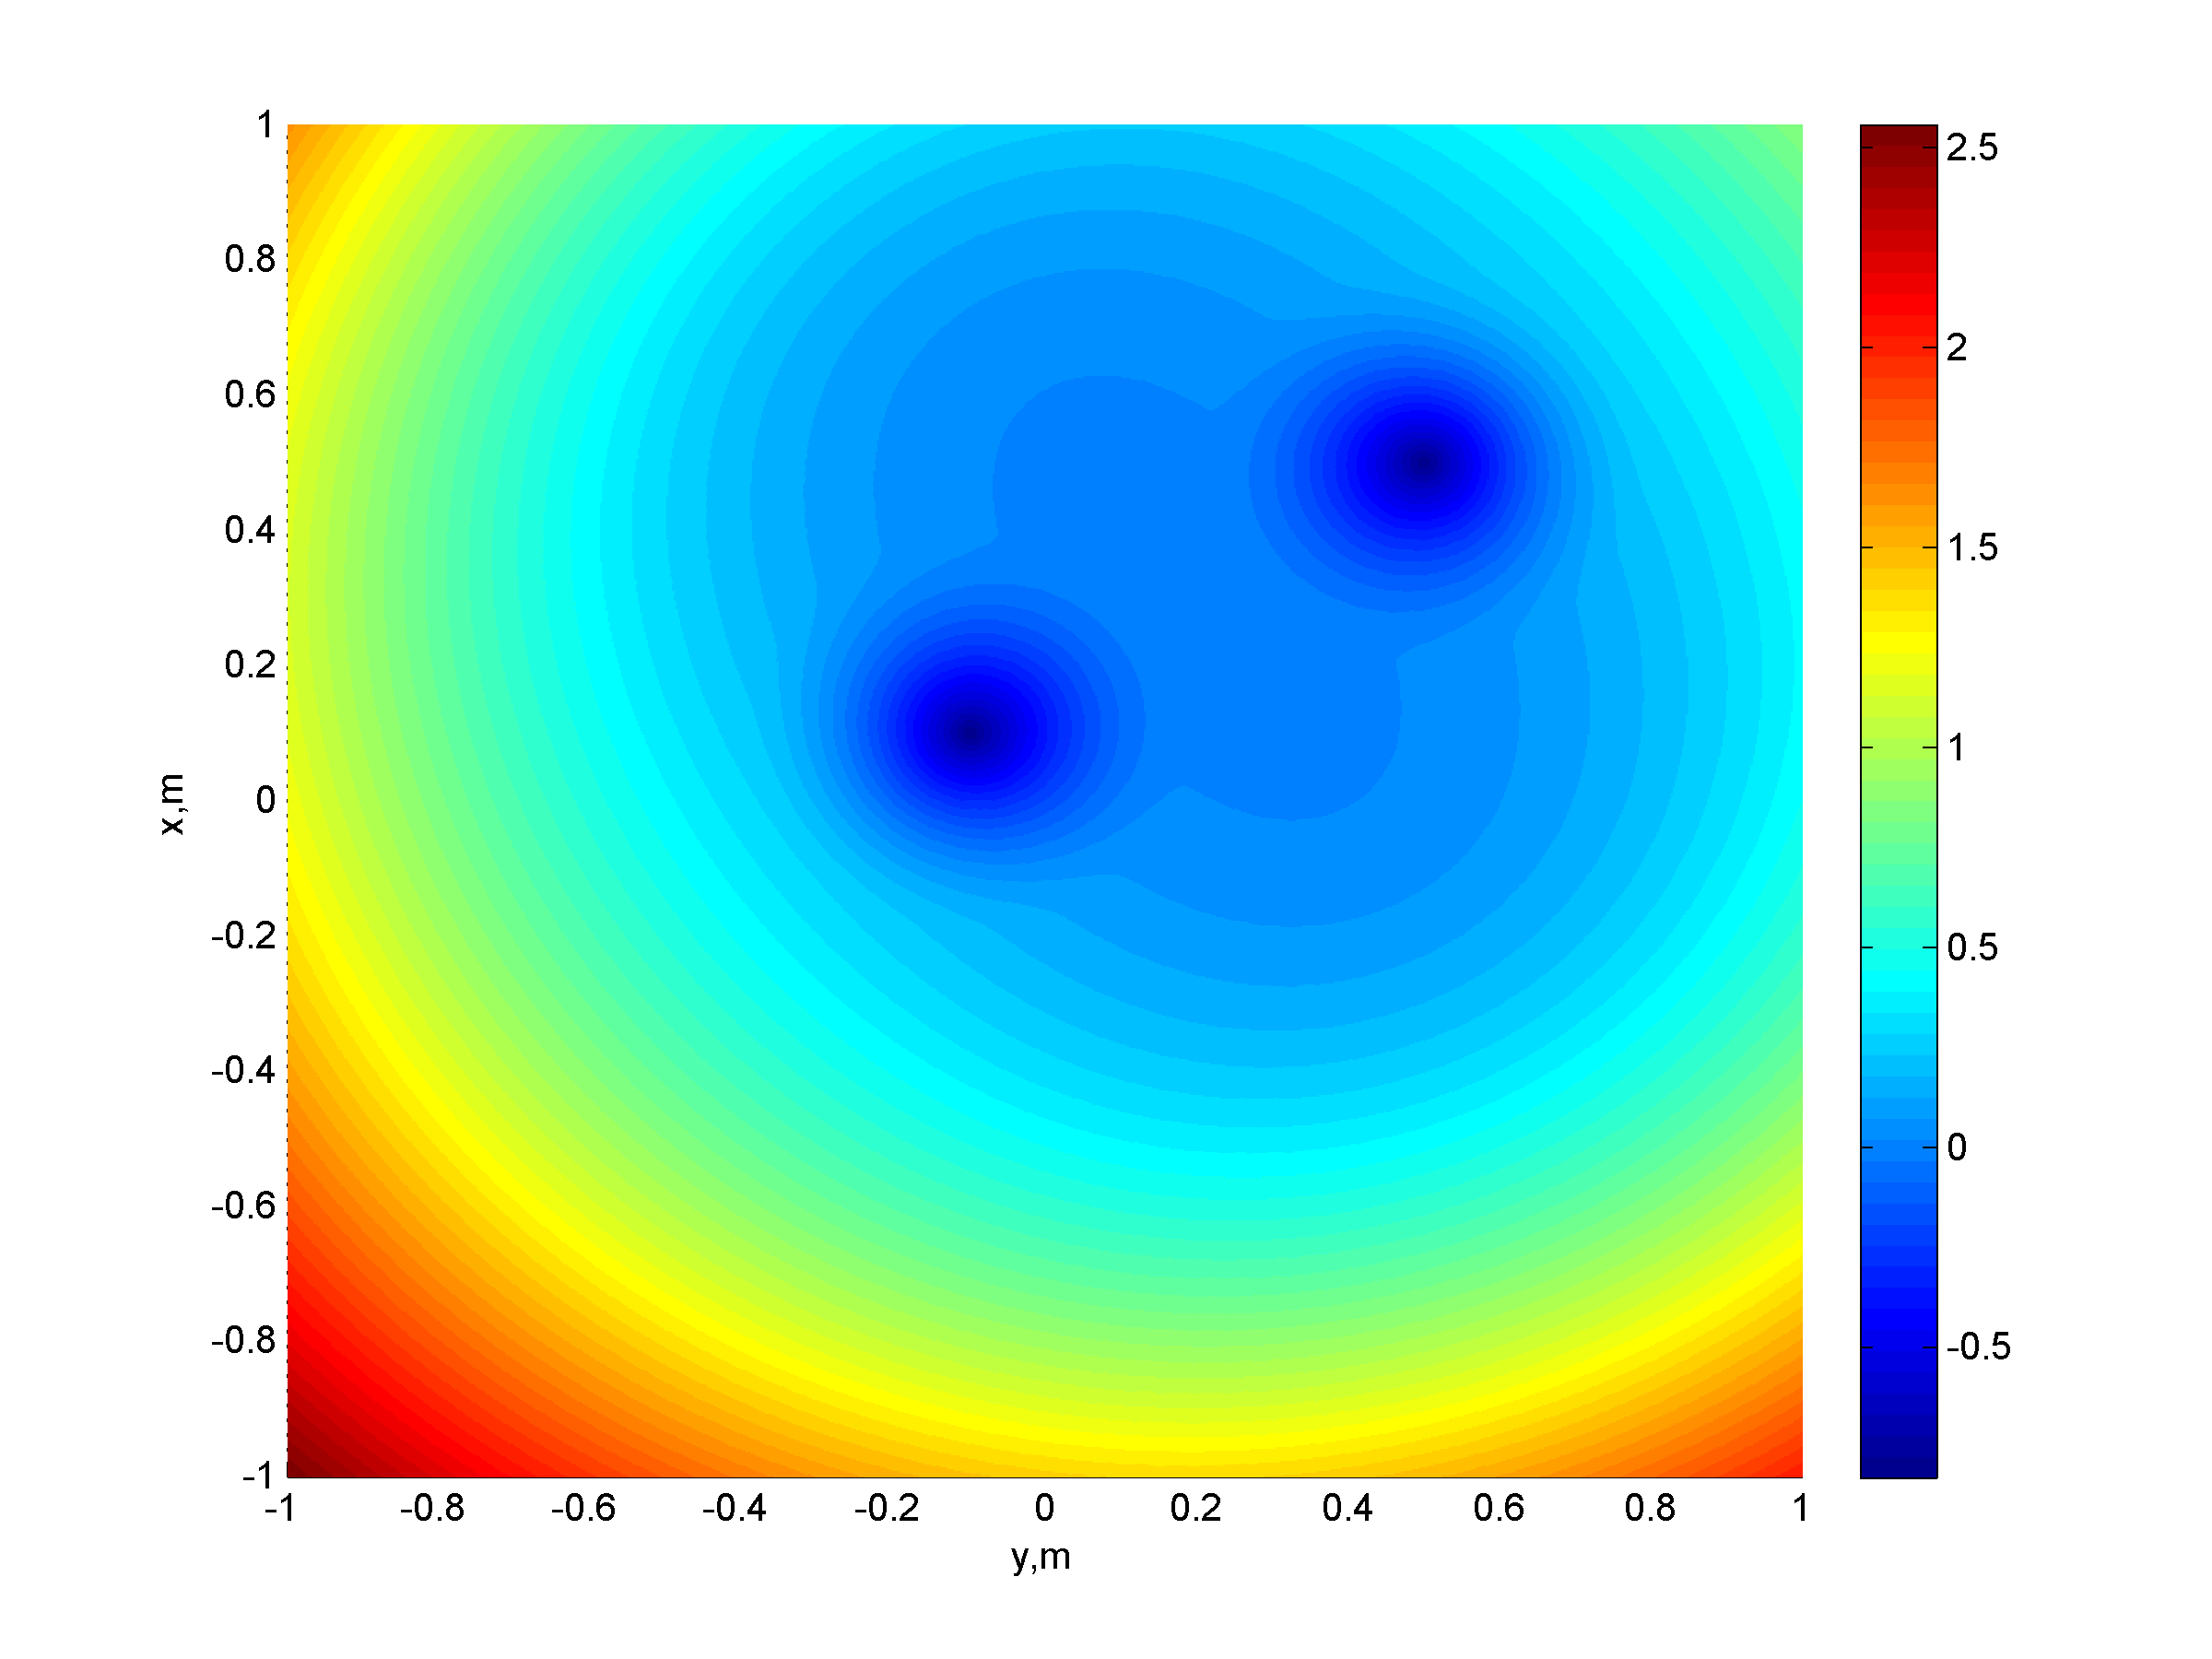
\includegraphics[width=\textwidth]{potential_field.png}}
					\caption{Potential-field around environmental obstacles.}
					\label{fig::potential_field}
				\end{figure}

			The biasing function $g_{\psi}(x)$ is used to weight the effect of individual scan points with respect to their relative angular location about the $z$-axis of $O_{L}$. $g_{\psi}(x)$ is parametrized by $\psi>0$, which defines a symmetric angular window. In \ref{eq::full_potential_fields}, $g_{\psi}(x)$ is selected as follows:
				\begin{eqnarray}
					\text{ang}\wrap{x} &=& \tan^{-1}\wrap{ \frac{\xcomp{x}}{\ycomp{x}} } \nonumber\\
					g_{\psi}(x) &=& 
					\begin{cases}
					\wrap{1-\abs{\frac{\text{ang}\wrap{x}}{\psi}}}^{\alpha_{g}}	& \text{ang}\wrap{x} < \psi \\
					0 	& \text{otherwise}.
					\end{cases}
				\end{eqnarray}
			where $\xcomp{x}$ and $\ycomp{x}$ are the $x$-axis and $y$-axis coordinates of the vector argument $x\in\RRe^{3}$; and $\alpha_{g}\leq1$ such that $g_{\psi}(x)$ is concave with respect to $\alpha_{g}$. This function is used to give priority to points which fall frontward of the robot and within the aforementioned angular window (of width $2\psi$) centered at the $y$-axis which emanates from $O_{L}$. To note: the $y$-axis of the frame $O_{L}$ always points in the direction of the robot's forward heading and emanates from the front of the LIDAR head. The reasoning for incorporating $g_{\psi}(x)$ is as follows: if the robot is heading forward and detects close-by obstructions at its sides (\IE at some angular location with an angular magnitude that is greater than or equal to $\abs{\frac{\pi}{2}}$), it is not necessary to perform an maneuvers to avoid these obstacles as they will not impede upon the robot's immediate forward motion, so long as they are sufficiently far from the robot's immediate workspace. The same is true for obstacles which are behind the robot, which will be completely disregarded according to the definition of $g_{\psi}(x)$ provided above. Only if the robot faces an obstacle which is directly ahead of it should it turn away to avert a potential collision. Thus, the parameter $\alpha_{g}$ in $g_{\psi}(x)$ is tuned to adjust the amount to which points are ``ignored" with respect to their angular distance from the front of the LIDAR head.

			%Considering only frontward points serves to reduce the potential for getting stuck in local minima, namely when the robot moves into an area where it faces equal potential from all sides. 
			%In the event that the robot does get stuck in a potential minima, a ``stuck" detection algorithm has been implemented. As the name suggests, this algorithm first detects if the robot is stuck in a local minima of the potential field based on a window of command histories.

			Finally, outputs of the potential field algorithm are mapped into forward and turning rate commands, ${v}_{L}^{r}$ and $\omega_{L}^{r}$, respectively, by the following control scheme:
				\begin{eqnarray}
					\theta_{L}^{r} 			&=& \tan^{-1}\wrap{ \frac{ \xcomp{\vec{u}^{r}_{L}} }{ \ycomp{\vec{u}^{r}_{L}} } } \nonumber\\
					\dot{v}_{L}^{r} 		&=& \beta_{v} \wrap{ P_{L} + v_{L,min}^{r} - v_{L}^{r} } \nonumber \\
					\dot{\omega}_{L}^{r} 	&=& \beta_{\omega} \wrap{ \wrap{ \frac{ \omega_{L}^{r,max} }{\pi} } \wrap{  \theta_{L}^{r} - \theta_{b,z} } - \omega_{L}^{r} }
				\end{eqnarray}
			where $\beta_{v}$ and $\beta_{\omega}$ are proportional-gain tuning parameters; $v_{L,min}^{r}>0$ is a small, minimum velocity used to prevent the robot from getting stuck in local minima; and $\theta_{b,z}$ is the robot's yaw in $O_{0}$. The parameters $\beta_{v}$ and $\beta_{\omega}$ can be viewed as \emph{update-inertias}, as they directly effect the influence of immediate commands on the overall forward velocity and turning rate of the robot. Furthermore, these gains can be used to low-pass updates to navigation parameters so as to remove jitter caused by degenerate LIDAR scans or sensor noise.


		\subsection{Simulated Potential-Fields Navigation Results}

				\begin{figure}[!h]
					\centering
					\fbox{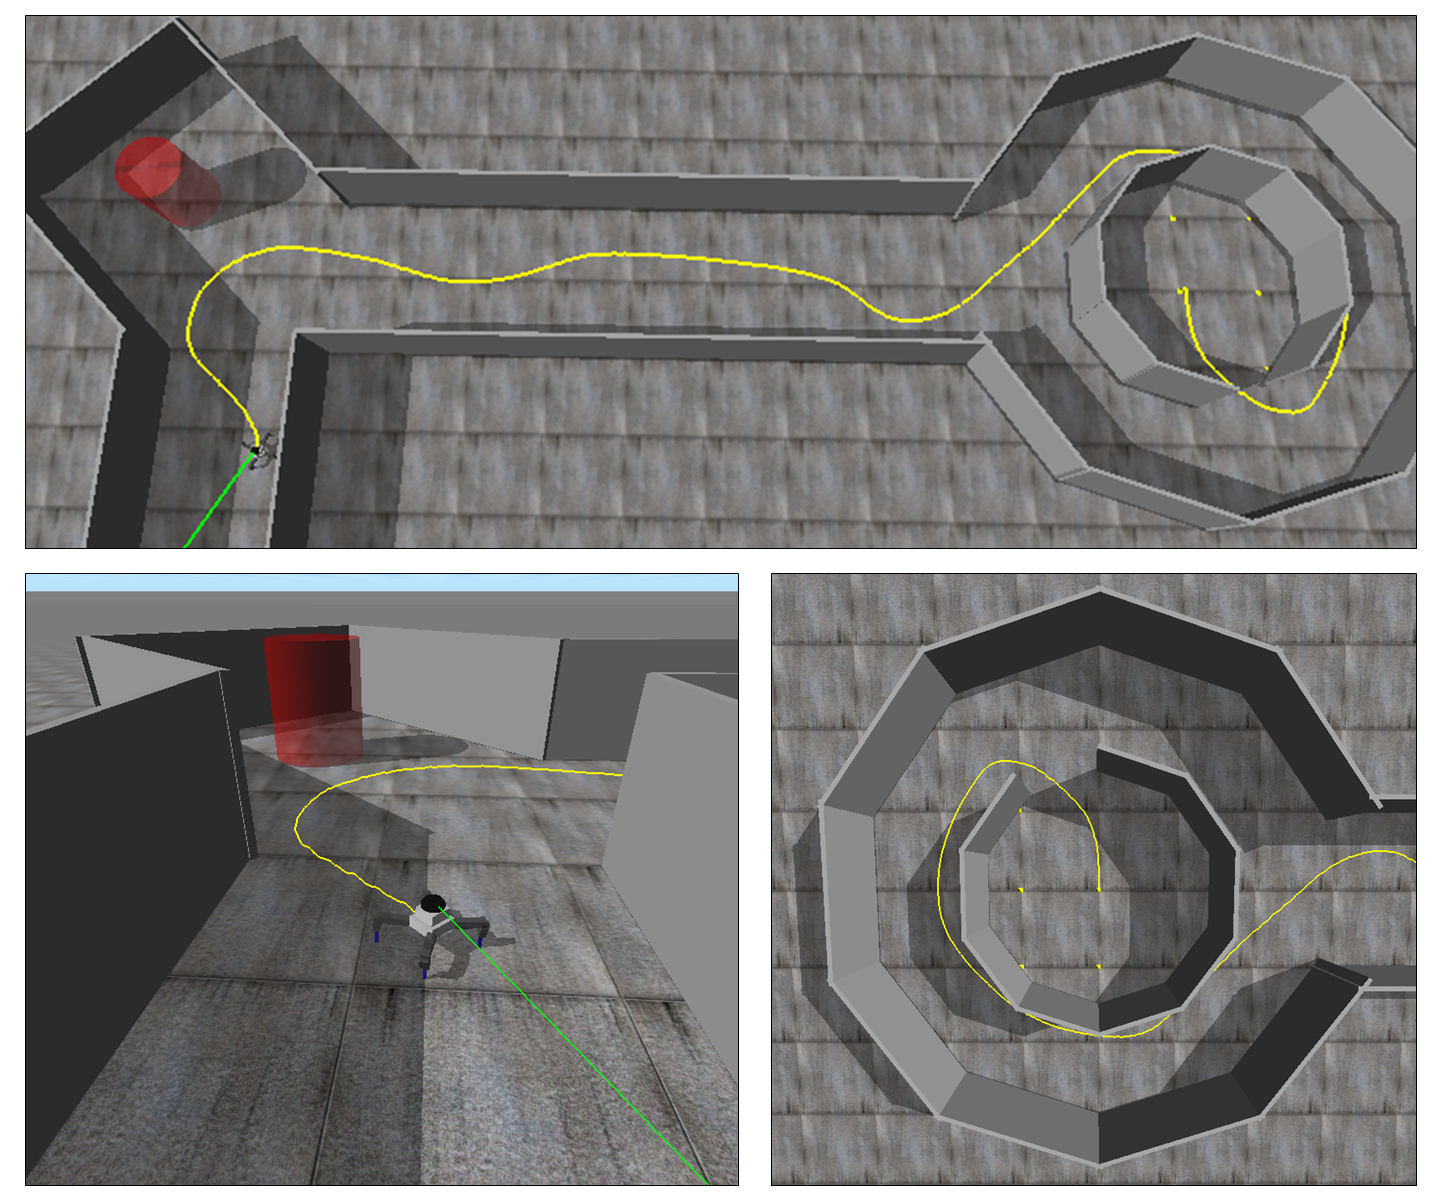
\includegraphics[width=\textwidth]{potential_field_full.png}}
					\caption{Path (shown in yellow) taken by robot through a simulated set of rooms and halls using the LIDAR-based potential-fields navigation scheme.}
					\label{fig::potential_field_results}
				\end{figure}
				\begin{figure}[!h]
					\centering
					\fbox{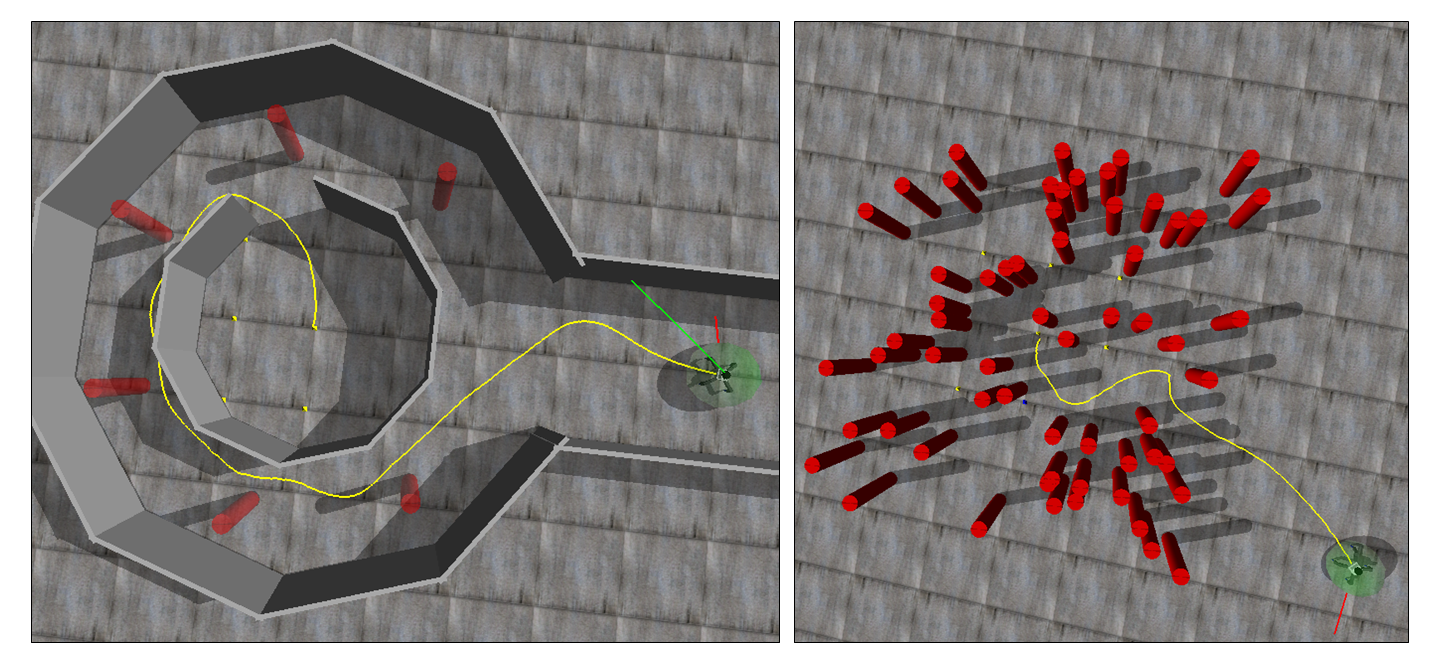
\includegraphics[width=\textwidth]{potential_field_full_obstacles.png}}
					\caption{Path (shown in yellow) taken by robot through a simulated set of rooms and obstacles.}
					\label{fig::potential_field_results_obstacles}
				\end{figure}
		
			Figure~\ref{fig::potential_field_results} shows the path resulting from a simulated trial in which the BlueFoot robot autonomously wandered through an environment, consisting of a room and several long corridors, using the described potential-fields mechanism. The simulated robot's trajectory is marked in yellow and shows that the robot was able to successfully navigate its immediate environment while avoiding collisions with the surrounding walls. Notably, the simulated robot naturally avoided smaller out-cove regions, which were mostly filled by cylindrical obstacles. This is because these regions had overwhelmingly lower potential relative to the longer corridor regions which were detected in the same immediate LIDAR frames. A second set of results is shown in Figure~\ref{fig::potential_field_results_obstacles} which highlights the robot's performance in environments additional obstacles. Likewise, the robot exhibits the desired obstacle-aversion performance using the potential-fields algorithm described. In both simulated trials, navigation parameters are set as follows: 
				$\alpha_{g}=0.25$,
				$\psi=\frac{\pi}{2}$,
				$d_{min}=0.5\text{ m}$,
				$\lambda_{c,1}=0.1$,
				$\lambda_{c,2}=10.0$, 
				$v_{L,min}^{r}=0.010\text{ }\frac{\text{mm}}{\text{s}}$
				$\omega_{L,max}^{r}=0.400\text{ }\frac{\text{rad}}{\text{s}}$
				and
				$\beta_{v}=\beta_{\omega}=0.1$.


		\subsection{Incorporation of Camera-Based Feature Tracking}
		
			Camera-based goal tracking is used in conjunction with the aforementioned potential-fields navigation scheme to move the platform through an environment while dynamically tracking targets which come into view of its camera. In this case, targets take the the form of features extracted from acquired images. The robot is guided towards these features using a visual-serving approach. 

			Trackable camera features can be generated in a variety of ways. For the purpose of BlueFoot's navigation, objects with distinct shapes or color have been chosen for tracking so that shape and blob detection algorithms can be employed to detect the relative positions of these features in BlueFoot's camera view. Namely, Hough Transform-based shape detection algorithms and color-blob detection algorithms from the Open Computer Vision library (OpenCV) are employed for the purpose of feature detection \cite{opencv_library}. Once detected, points representing the centers of each feature, relative to the 2D camera frame, are mapped into forward velocity and turning rate commands. These commands are used to control the robot such that the center of the detected feature is aligned with the center of each image fame. These camera-based commands are then mixed with the outputs of the potential-fields controller as a weighted sum to form a hybrid navigation control law.

			The visual-servoing approach to be described is agnostic of the type of feature being tracked. Namely, this approach relies on the relative position of the center of each feature, represented as a pixel-position, $p_{Im} = [u,v]^{T} \in \mmathbb{Z}^{2}$ in the 2D image frame, $O_{Im}$, and a relative size, $r$, measured in pixels. In the case of circular features, for example, $r$ represents the radius of the detected circle. For color-blob features, $r$ represents the radius of a circle which fully inscribes the colored object.

			For the purpose of target tracking, it is desired that the robot's forward speed be controlled proportionally to the robot's relative closeness to the object of interest. A measure of closeness is determined from the value $r$ associated with a particular feature. Namely, it is desired that the robot stops when it becomes \emph{close enough} to the target object, and faster towards the feature when it is in sight, but further away. This control law is imposed to prevent the robot from crashing into the target being tracked. The position of a feature's center is used to control the robot's turning rate, as well as the commanded pitch of the robot's trunk, $\theta_{b,x}^{r}$. Trunk articulation important during feature tracking routing as it aids in keeping the tracked-target objects centered in the image frame. Provided that the target is moving slower than the what the system can track, this will ensure the target remains in sight at all times.

			A separate set of navigation commands, $v_{C}^{r}$ and $\omega_{C}^{r}$; and an additional body-pitching command, $\theta_{b,x}^{r}$,  are generated from an extracted feature location, $p_{Im} = [u,v]^{T}$ (in the image frame $O_{Im}$) as follows: 
				\begin{eqnarray}
					v_{C}^{r} 			& = & v_{C}^{r,max} \wrap{ 1 - e^{ -c_{r} \wrap{ r-r_{min} }^{2} } } 	\nonumber 	\\
					\omega_{C}^{r} 	& = & \omega_{C}^{r,max} \wrap{\frac{ w_{Im} - 2 u  }{ w_{Im} } }		\nonumber 	\\
					\theta_{b,x}^{r}	& = & \theta_{b,x}^{r,max} \wrap{ \frac{ 2 v - h_{Im} }{ h_{Im} } } 		
				\end{eqnarray}
			where $v_{C}^{r,max}$, $\omega_{C}^{r,max}$ and $\theta_{b,x}^{r,max}$ are the maximum magnitudes of forward velocity, turning rate, and body-pitching commands, respectively; $c_{r}$ is a sensitivity parameter; $r_{min}$ defines a minimum feature size which will result in the administration of a zero velocity command, $v_{C}^{r,max}=0$, to the platform; and $w_{Im}$ and $h_{Im}$ define the width and height, respectively, of the image being processed. Having now established a formulation for how a single, distinct, feature is used to guide the platform towards a target, a means of fusing the LIDAR-based command signals and the camera-based command signals will be defined.

				\begin{figure}[!h]
					\centering
					\fbox{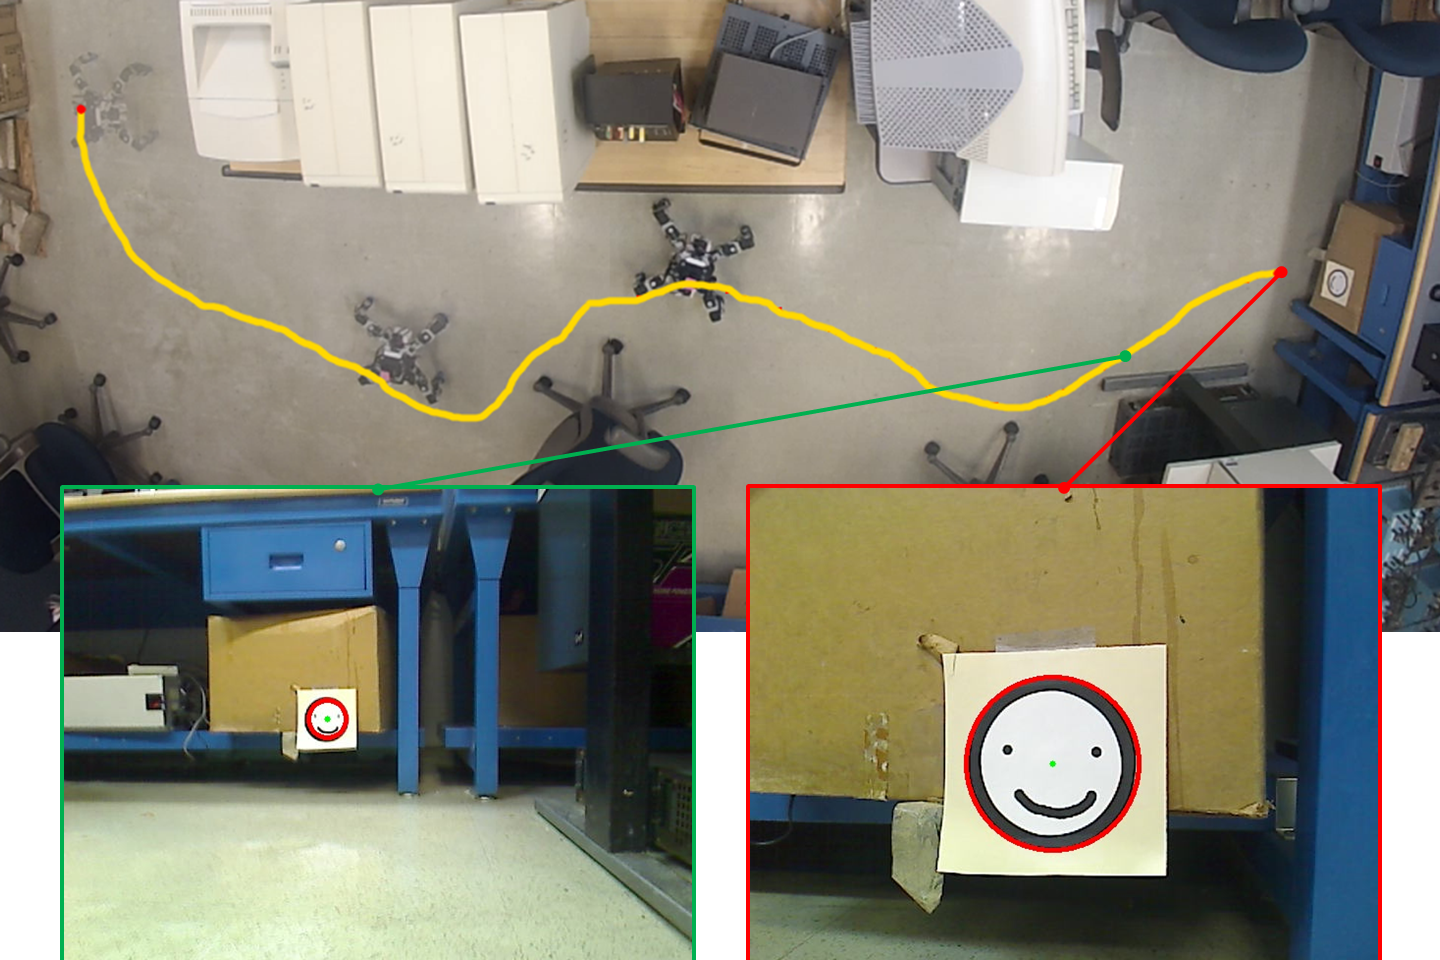
\includegraphics[width=\textwidth]{potential_field_full_real.png}}
					\caption{Path (shown in yellow) taken by robot through a real-world lab setting showing the robot's view of the goal marker.}
					\label{fig::potential_field_results_real}
				\end{figure}

			The composition of this hybrid command technique is motivated by two related subtasks: 
				\begin{enumerate}
				\item to use the potential-fields algorithm during a wandering phase, when a target object is not in sight and
				\item to guide the robot safely towards a target once in sight.
				\end{enumerate}
			Moreover, camera-based tracking commands will have a greater influence on system navigation (through the variables $v^{r}$ and $\omega^{r}$) as the platform becomes closer to the desired target. A straight-forward way to achieve this is to use the relative size, $r$, of tracked features in the image frame, as will be described. With this in mind, a command-mixing scheme is defined as follows:
			\begin{eqnarray}
				v(r) &=&
				\begin{cases}
				e^{ -c_{mix} \wrap{ r - r_{mix}}^{2} } 	& \text{if } r < r_{mix}	\\
				1											& \text{otherwise}
				\end{cases}
								\nonumber \\
						\left[\begin{array}{c} v^{r} 	\\ \omega^{r} 		\end{array} \right] &=& 	
				v(r)	\left[\begin{array}{c} v^{r}_{C}\\ \omega^{r}_{C} 	\end{array} \right] + 
				(1-v(r))\left[\begin{array}{c} v^{r}_{L}\\ \omega^{r}_{L} 	\end{array} \right] 
			\end{eqnarray}
			where $c_{mix}$ is a sensitivity parameter; and $r_{mix}$ defines a registered feature size which will cause the robot shift full priority to the camera-based navigation scheme. The reasoning for such an approach hinges on the assumption that when the platform is further away from a goal, there is a higher probability that it will encounter an obstacle. Conversely, when the goal becomes closer to the platform, it is assumed that the number of obstacles between the robot and the target is small, making it safer to promote the importance of reaching the target in sight. It is defined that if a feature is not visible within the current view of the camera, then $r=0$.

			Figure~\ref{fig::potential_field_results_real} shows the robot's path through a real-world environment. In this trial, the robot is setup to detect a circular target marker which is placed such that it will fall into the robot's gaze. The efficacy of this navigation scheme is highlighted, particularly, when the robot successfully rounds a chair in its way. Additionally, the robot successfully detects and reaches a target marker. The robot's view of the target marker from further away and upon reaching the target are also shown in this figure. In each image, the perimeter and center of the target marker are highlighted to show the feature characteristics determined by the robot.






	\section{Towards Rough Terrain Navigation}

		\subsection{Terrain Mapping from 2D Scans}
			\label{ssec::terrain_mapping}
			\begin{figure}[!h]
				\centering
				\fbox{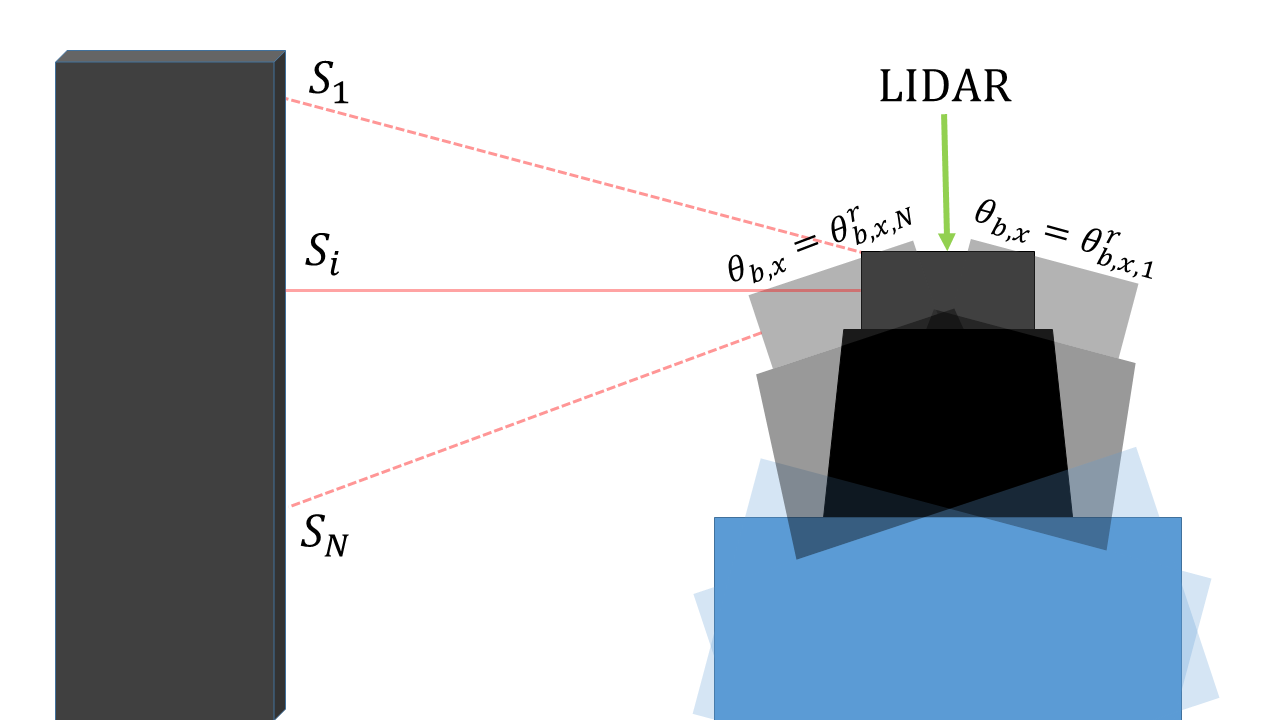
\includegraphics[width=\textwidth]{laser-sweep.png}}
				\caption{LIDAR swept over a range of angles, $\theta_{b,x} \in [\theta_{b,x,1}^{r},\theta_{b,x,N}^{r}]$. }
				\label{fig::sensor_sweep}
			\end{figure}
			The BlueFoot platform composes 3D point clouds from a series of 2D LIDAR scans and associated trunk orientation estimates, $\hat{\theta}_{b}$, which are generated using a calibrated EKF routine. LIDAR articulation is achieved by slowly pitching the trunk over an angular range $\theta_{b,x}\in[-\theta_{s,min},\theta_{s,max}]$ while keeping the platform's feet planted. The angular trajectory of $\theta_{b,x}$ is discretized into $K$ divisions, which defines the number scan-levels used in composing a 3D cloud, and further, an angular scan resolution about the $x$-axis. The rate of scan completion is dependent upon the spinning rate of the LIDAR. Furthermore, the pitch of the trunk is controlled during a scanning routine as follows:
				\begin{equation}
					\begin{split}
					\theta_{b,x,k}^{*} &= 
						\wrap{\theta_{s,max}-\theta_{s,min}}
							\wrap{\frac{k}{K}} + 
								\theta_{s,min} \\
					\dot{\theta}_{b,x}^{r} &=
						\alpha_{\theta}
							(\theta_{b,x,k}^{*} - \hat{\theta}_{b,x} ) \\
							\forall k &\in \{1,...,K\}
					\end{split}
				\end{equation}
			where $k$ is a step-counter which is incremented each time the LIDAR completes a full scan cycle; and $\alpha_{\theta}$ is a scalar, proportional gain factor. Given this formulation, the approximate rate of completion for a full 3D-scan, $\tilde{f}_{scan}$, is as follows:
				\begin{equation}
					\tilde{f}_{scan}\approx\frac{1}{K}\frac{\Delta\theta_{L}}{\omega_{L}}
					\label{eq::point_cloud_collection_rate}
				\end{equation}
			where $\Delta\theta_{L}$ and $\omega_{L}$ are the angular range and spinning rate of the LIDAR, respectively.

			As previously mentioned, particular trunk configurations are achieved as a aggregation of leg configurations. The inverse kinematic solution for each leg is solved, incorporating a desired trunk position and orientation, yielding a controlled trunk pose, as defined in Section~\ref{sec::inverse_position_kinematics}. Moreover, the sweeping (pitching) range which BlueFoot can achieve during a scanning sequence is limited by the kinematic-feasibility of each \Kth trunk pose that must be attained. For example, BlueFoot can pitch which cover a range of $\pm 30\text{ degrees}$ when configured in its default stance (see Table~\ref{tab::DefaultStance}).

			A single scan is taken at each \Kth pose of the sweeping trajectory. The newly acquired scan is transformed from the LIDAR sensor frame, $O_{L}$, to the world frame, $O_{0}$, by a homogeneous transformation $H^{L}_{0}$ which is defined as follows
				\begin{equation}
					H^{L}_{0} = H^{L}_{b} H^{b}_{0}
					\label{eq::world_to_sensor}
				\end{equation}
			where $H^{b}_{0}$ is a transformation from $O_{0}$ to the trunk frame $O_{b}$, as defined in Chapter~\ref{ch::system_modeling}; and $H^{L}_{b}$ defines a transformation from the frame $O_{b}$ to the LIDAR frame, $O_{L}$. $H^{L}_{b}$ is necessary for knowing the position of the LIDAR head with respect world frame, as the sensor itself has some offset and rotation relative to the robot's body. Each 2D point from $x_{i} \in \emph{S}$ from a raw LIDAR scan, $\emph{S} \subset \RRe^{2}$, is transformed into a 3D scan segment, $\bar{S}_{k} \subset \RRe^{3}$, with respect to the frame $O_{0}$ by:
				\begin{equation}
					\left[
						\begin{array}{c}
							\bar{x}_{i,k} \\ 1
						\end{array}
					\right]
				 = H^{L}_{b} H^{b}_{0}	
					\left[
						\begin{array}{c}
							x_{i} \\ 0 \\ 1
						\end{array}
					\right] \forall x_{i} \in \emph{S}
					\label{eq::scan_to_segment}
				\end{equation}
			where $\bar{x}_{i,k} \in \bar{S}_{k}$ is a point within the \Kth 3D scan segment $\bar{S}_{k}$. After the sweeping routine is complete, 3D scan segments are composed into a final point cloud, $\bar{S}$ by:
				\begin{equation}
					\bar{S} = \bigcup_{k=1}^{N_{s}} \bar{S}_{k}
					\label{eq::scan_composition}
				\end{equation}
			where $N_{s}$ defines the number of scans taken during the sweeping routine. For the sake of simplicity, it is assumed that the trunk's position, $p_{b}$, is fixed and the body is completely ridged during a 3D scanning routine (\IE $\dot{p}_{b}=0$). In the results to be presented, it will be shown that this is a reasonable assumption, as the robot is not walking and the trunk is pitched sufficiently slowly over the angular sweeping range. A slow sweep rate ensures that perturbations caused by vibrations during trunk rotation are small, and thus do not cause for significant deviations in LIDAR scan points. These vibrations result mainly from foot slippage and actuator noise.
				\begin{figure}[!h]
					\centering
					\fbox{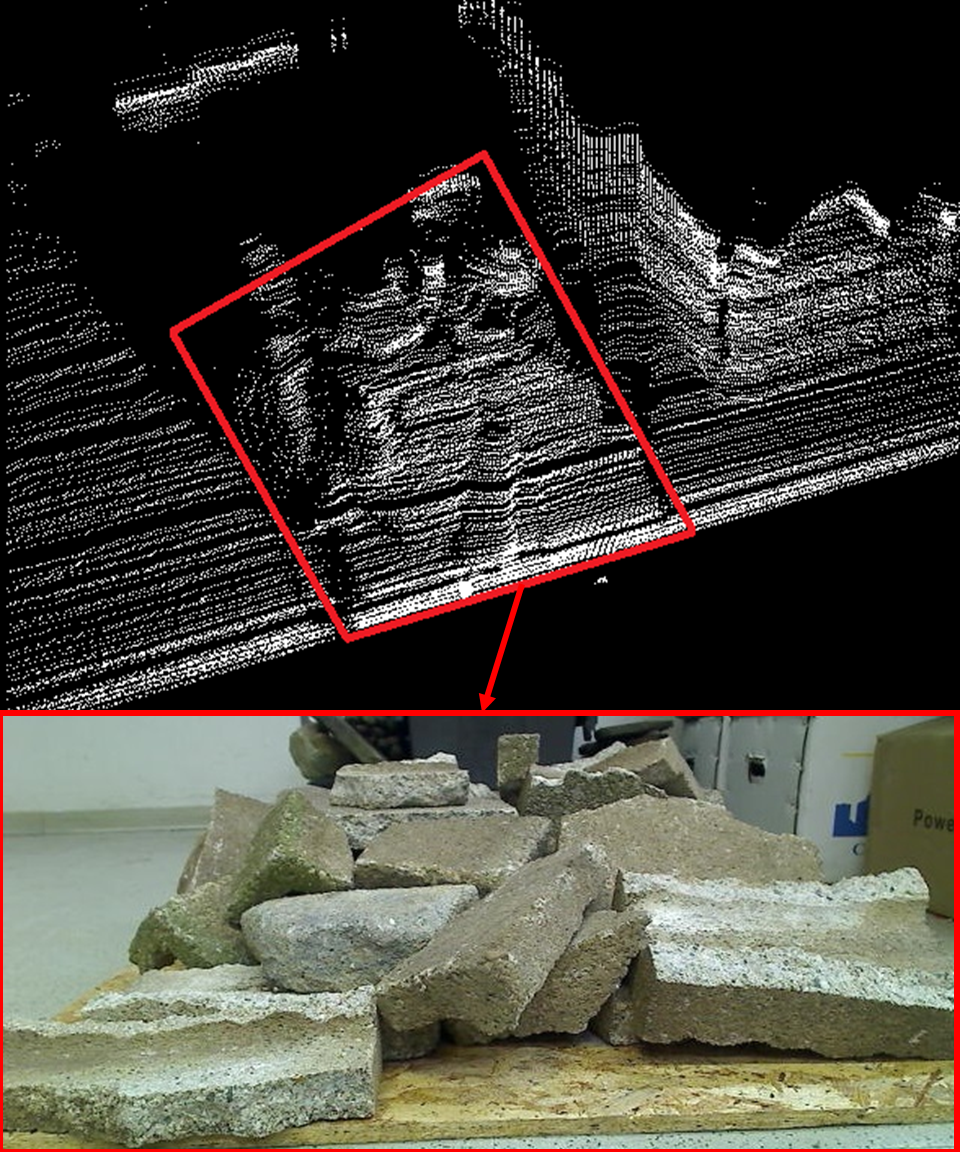
\includegraphics[width=1.0\textwidth]{rough_terrain.png}}
					\caption{Original 3D point-cloud of terrain patch \emph{(top)} and corresponding view from robot's on-board camera \emph{(bottom)}.}
					\label{fig::pointcloud_terrain_patch}
				\end{figure}




		\subsection{Height-Map Generation from a 3D Point Cloud}
			
			3D point clouds can be converted into height-maps to represent surfaces. Here a height-map will be represented via an associated discrete space $\mmathbb{Z}^{\mmathcal{M}}\subset\mmathbb{Z}^{2}$ with a coordinate system $O_{\mmathcal{M}}$. Height-map representations are convenient for use in planning as they can be used to assign costs to path transitions in a straightforward way. Height-map information is represented as a matrix $\mmathcal{M}\in \RRe^{n\times m}$ with height elements $m_{i,j}$. A set of indices $\bar{p} = \{i,j\}\in\mmathbb{Z}^{\mmathcal{M}}$ is used to refer to the element $m_{i,j}$ in $\mmathcal{M}$ and, simultaneously, a planar location with respect to the $O_{\mmathcal{M}}$ frame. Thus, the notations $m_{i,j}$ and $\mmathcal{M}(\bar{p})$ will be used interchangeably to represent a height stored in the height-map matrix $\mmathcal{M}$.

			To create the height-map, a $w\times d$ region of interest (ROI) with a relative location $\bar{p}_{0}^{ROI}$ in $O_{0}$ is first selected. This region is then discretized in $(nm)$ subregions. The dimensions $w$ and $d$ of the ROI represent lengths along $x$-axis and $y$-axis respectively. The notation $\mmathbb{R}^{\mmathcal{M}}\subset \RRe^{3}$ will be used to represent the set of points contained within the ROI.  Moreover, the space $\mmathbb{Z}^{\mmathcal{M}}$ is used to represent a discretized analogue to $\mmathbb{R}^{\mmathcal{M}}$, where each position $\{i,j\}\in\mmathbb{Z}^{\mmathcal{M}}$ represents the \Ith, \Jth subregion of the ROI. Moreover, each subregion has an associated height of $m_{i,j}$ stored in $\mmathcal{M}$. An ROI selected from a source point cloud $\bar{S}$ will be represented as $\bar{S}_{ROI}\subset\RRe^{3}$. It is assumed that the location, $\bar{p}_{0}^{ROI}$, and size of this ROI are determined via some auxiliary detection algorithm. Such a detection algorithm: 
			\begin{enumerate}
				\item selects an area with high terrain variation (large changes in gradient),
				\item determines $\bar{p}_{0}^{ROI}$,
				\item and determines the bounding region of the ROI.
			\end{enumerate}%%%
			For the results shown in this section, an exemplary ROI has been manually selected from an existing 3D point cloud. An algorithm which fulfills the above mentioned detection requirements has yet to be fully explored under the scope of this project. %Such an algorithm would need to involve mechanisms for point cloud segmentation and feature evaluation. Additionally, images of the the robot's immediate terrain could be used to aid in this process by locating areas with high feature density incurred by terrain variations.

			The point $\bar{p}\in\mmathbb{Z}^{\mmathcal{M}}$ is used to represent the location of a discrete subregion that is $(w/m) \times (d/n)$ area. A corresponding height for that subregion is stored in $m_{i,j}$, and is selected as the largest $z$-component of any point that falls within said subregion. The transformation from a point cloud element, $\bar{x}$, to an element within the discretized height-map frame can be described by:
				\begin{equation}
					\left[
						\begin{array}{c}
						\bar{p} \\
						m_{i,j}  	\\
						\end{array}
					\right]
					=
					\left[
						\begin{array}{c}
						i \\
						j \\ \hline
						m_{i,j}  	\\
						\end{array}
					\right]
					=
					\ciel{
						\left[
							\begin{array}{ccc}
							n/d & 0 	& 0 \\
							0 	& m/w 	& 0 \\
							0 	& 0 	& 1 \\
							\end{array}
						\right]
						\wrap{
							\left[
								\begin{array}{ccc}
								0 &-1 & 0 \\
								1 & 0 & 0 \\
								0 & 0 & 1 \\
								\end{array}
							\right]
							\wrap{\bar{x}-\bar{p}_{0}^{ROI}}
							+
							\left[
								\begin{array}{c}
								d \\
								0 \\
								0 \\
								\end{array}
							\right]
						}
					}
					\label{eq::toheightmapframe}
				\end{equation}
			where $\ciel{*}$ is an element-wise ceiling function which takes a vector argument $(*)$.

			Depending on the density of the source point cloud, the basic height-map conversion process has the potential to produce relatively sparse height-maps. To deal with this, a dilation and smoothing routine is used to fill in gaps in $\mmathcal{M}$. During dilation, each non-zero height element within the map is expanded into a region around an existing element \cite{opencv_learn_immorph}. Dilation parameters are tuned so that uniform surface representation with minimal gaps between non-zero height elements is achieved. Finally, a median filter is applied to the dilated height-map to smooth transitions between elements.
			\afterpage{%
				\begin{figure}[!t]
					\centering
					\fbox{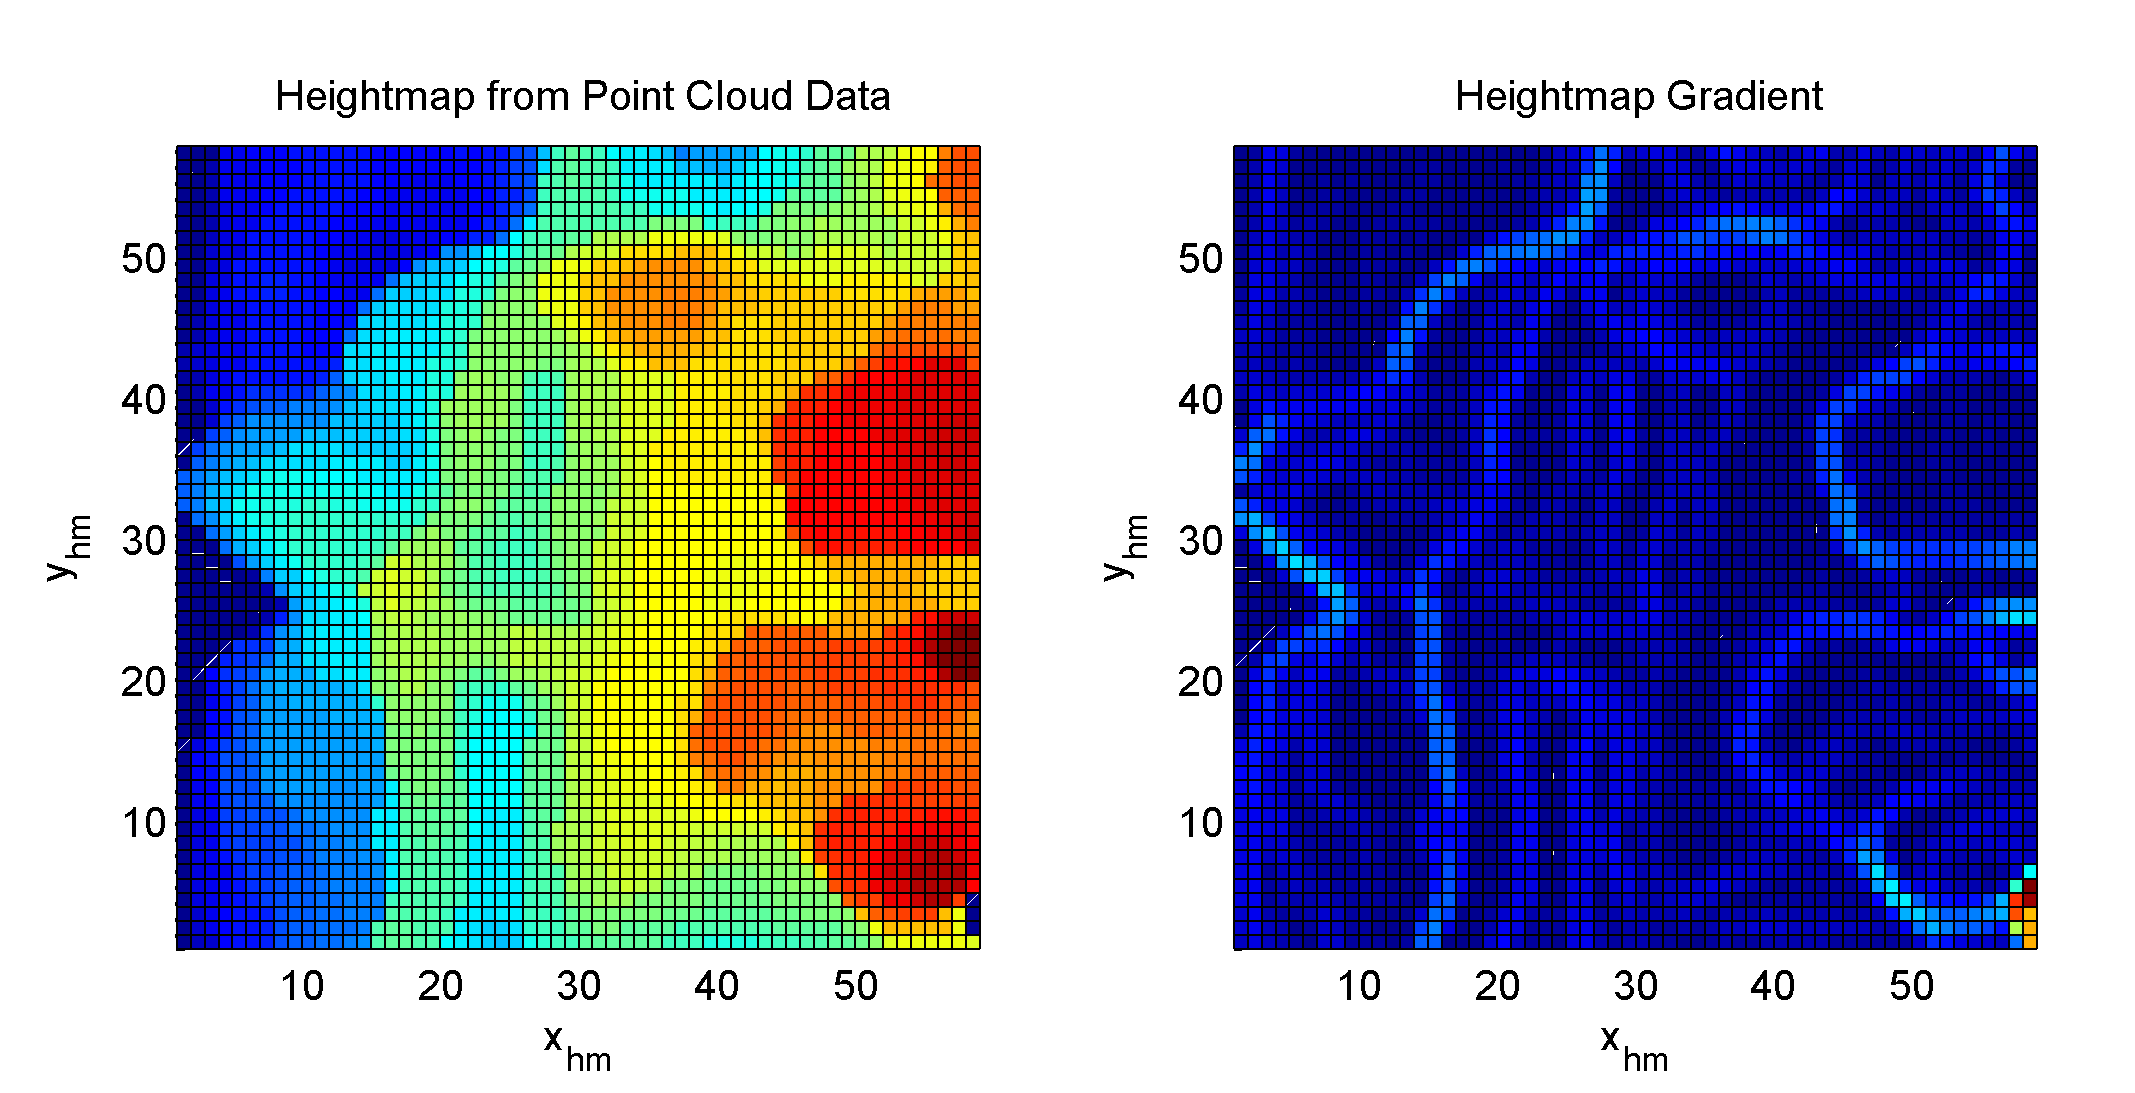
\includegraphics[width=\textwidth]{terrain_grad_crop.png}}
					\caption{A height-map \emph{(left)} and its corresponding gradient \emph{(right)}.}
					\label{fig::heightmap_terrain_patch}
				\end{figure}
				\begin{figure}[!t]
					\centering
					\fbox{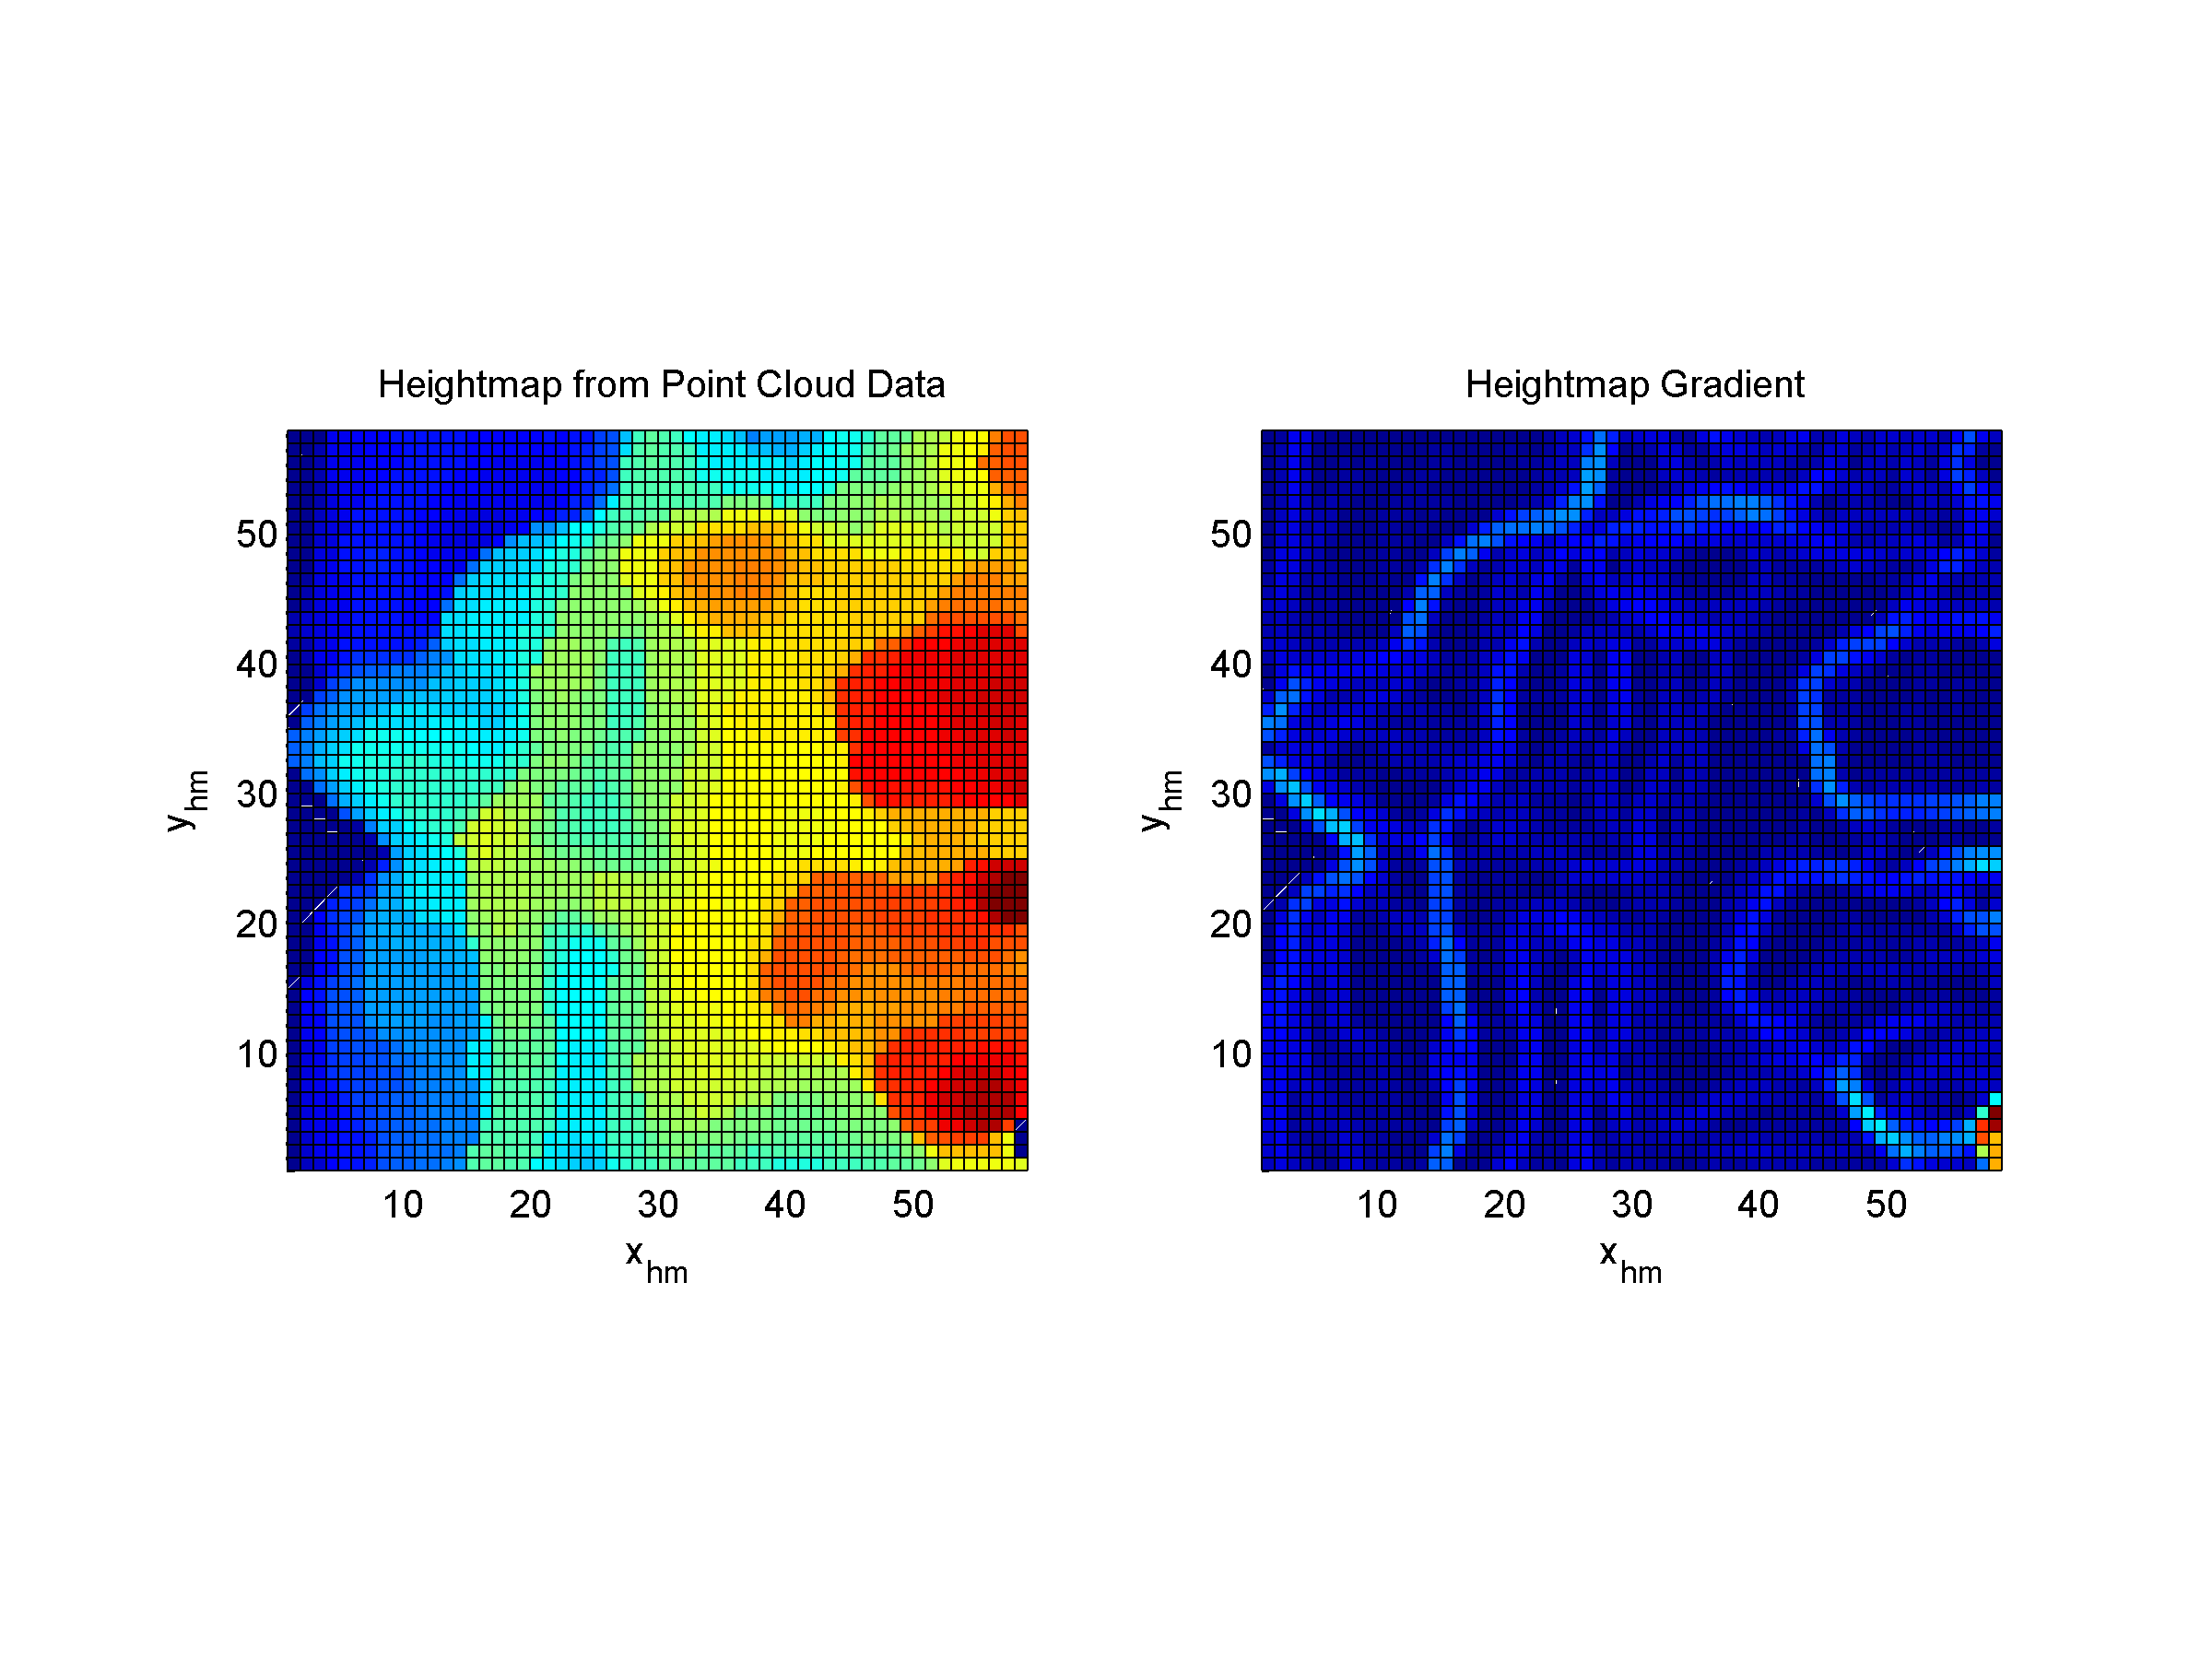
\includegraphics[width=\textwidth]{terrain_4545.png}}
					\caption{Height-map showing terrain variation.}
					\label{fig::heightmap_terrain_patch_ortho}
				\end{figure}
			\clearpage}

			The full height-map conversion process (from a 3D point cloud) is summarized in Algorithm~\ref{alg::hmconvert}. In this algorithm, $\emph{\text{isolateROI}}$ represents a function which locates a region of interest within the point cloud $\bar{S}$; $\emph{\text{subdivIndex}}$ performs the transformation in $\ref{eq::toheightmapframe}$, which generates indices $(i,j)\in\mmathbb{Z}^{\mmathcal{M}}$ corresponding to a point in $O_{0}$; $\emph{\text{dialateFeatures}}$ performs a calibrated image-dilation routine; and $\emph{\text{medianFilter}}$ performs a standard image median filter routine with a $w\times w$ window size. Once a height-map has been generated, a corresponding gradient, as shown in Figure~\ref{fig::heightmap_terrain_patch}, is generated using a Sobel image gradient operation (from OpenCV). The image gradient operation is represented by the function $\emph{\text{imageGradientSobel}}$.

			\begin{algorithm}[!h]
				\begin{algorithmic}
					\State{\textbf{init} $\mmathcal{M} = 0, \nabla\mmathcal{M}, m, n, w, d, \bar{S},\bar{p}_{0}^{ROI}$}
					\State{$\{\bar{S}_{ROI},\bar{p}_{0}^{ROI}\} = \text{isolateROI}(\bar{S})$}
					\ForAll{$\bar{x}_{k}\in \bar{S}_{ROI}$}
						\State{$[i,j] = \text{subdivIndex}(\xcomp{\bar{x}_{k}},\ycomp{\bar{x}_{k}},\bar{p}_{0}^{ROI},w,d,m,n)$}
						\If{$\zcomp{\bar{x}_{k}} > m_{i,j}$}
							\State{$m_{i,j} \leftarrow \zcomp{\bar{x}_{k}}$}
						\EndIf
					\EndFor
					\State{$\mmathcal{M} \leftarrow \text{dialateFeatures}(\mmathcal{M})$}
					\State{$\mmathcal{M} \leftarrow \text{medianFilter}(\mmathcal{M},w)$}
					\State{$\nabla\mmathcal{M} = \text{imageGradientSobel}(\mmathcal{M})$}
				\end{algorithmic}	
				\caption{3D ROI point cloud to height-map conversion.}
				\label{alg::hmconvert}
			\end{algorithm}






		\subsection{An Approach for Cost Assignment from a Height-Map}

			A discrete height-map space can be converted to a cost representation for the purpose of foot-placement planning over rough terrain. Here, a cost-tensor, $\mmathcal{C}\in\RRe^{n\times m\times l}$, is used to represent a discrete cost space. Each element $c_{i,j,u}$ in $\mmathcal{C}$ represents a transition cost for a particular location $(i,j,u)$. The first and second dimensions of $\mmathcal{C}$ (of size $n$ and $m$) directly correspond to the width and depth of the discretized height-map space $\mathbb{Z}^{\mmathcal{M}}$. The third dimension represents a discretization of the robot's yaw state, $\theta_{b,z}\in[-\pi,\pi]$ into $l$ subdivisions.  In the sections to follow, the notation $\mmathcal{C}(\bar{p}^{\mmathcal{M}},u)$ and $\mmathcal{C}(i,j,u)$ will be used interchangeably to refer to a cost-element, $c_{i,j,u}$, from the transition-cost tensor $\mmathcal{C}$.


			The mapping between a height-map,  $\mmathcal{M}$, and cost-tensor, $\mmathcal{C}$, is represented as follows:
				\begin{equation}
					\setwrap{ \mmathcal{C} = f(\mmathcal{M},\Gamma)\text{ }:\text{ }\RRe^{n\times m} \rightarrow \RRe^{n\times m \times l} }
					\label{eq::cost_mapping}
				\end{equation}
			where $\Gamma$ is a static configuration matrix used to describe the nominal spacing between the robot's feet. $\Gamma$ is composed as follows:
				\begin{equation*}
					\Gamma = \setwrap{\bar{p}_{1,e}^{\mmathcal{M}},\bar{p}_{2,e}^{\mmathcal{M}},\bar{p}_{3,e}^{\mmathcal{M}},\bar{p}_{4,e}^{\mmathcal{M}}}
					\label{eq::cost_gamma}
				\end{equation*}
			where $\bar{p}_{v,e}^{\mmathcal{M}}=[i_{v},j_{v}]^{T}\in\mmathbb{Z}^{\mmathcal{M}}$ represents the position of each $v^{th}$ foot in the height-map space with $i_{v}\in \setwrap{1,...,n}$ and $j_{v}\in\setwrap{1,...,m}$. By formulating cost with respect to static foot configurations, planning is simplified to finding a trajectory for body position. Target foot positions are then generated relative to planned body locations during trajectory execution using $\Gamma$ and \ref{eq::rel_feet}, to follow. The mapping, $f(\mmathcal{M},\Gamma)$, has been formulated with respect to three main cost elements:
				\begin{enumerate}
					\item variation in height between all current footholds
					\item terrain steepness around any foothold
					\item and net robot rotation at each path-step.
				\end{enumerate}
			The first cost element is chosen to penalize configurations in which the robot must stand on non-level terrain. This aids in ensuring that the kinematic workspace of each leg is not compromised by reducing the amount of ``stretching" the robot has to perform in order to attain a particular configuration atop the terrain. The second cost element is used deter the robot from attempting to plan footholds atop overly steep terrain. The final cost element is used to ensure the robot does not plan to perform any large changes in direction while traversing the terrain, which could cause for needless motion (perhaps even loops) in the planned path. 

			To perform the conversion between $\mmathcal{M}$ and $\mmathcal{C}$, a \emph{moving} foothold matrix $\Gamma'(\bar{p}^{\mmathcal{M}}_{b},u) \in \mmathbb{Z}^{2\times4}$ is first defined as follows:
				\begin{equation}
					\Gamma'(\bar{p}^{\mmathcal{M}}_{b},u) = \ciel{ R_{z}^{\mmathcal{M}}(\gamma(u))\Gamma } + \bar{p}^{\mmathcal{M}}_{b} B \\
					\label{eq::rel_feet}
				\end{equation}
			where  $\bar{p}^{\mmathcal{M}}_{b} = [i,j]^T\in\mmathbb{Z}^{\mmathcal{M}}$ and $u \in \setwrap{1,...,l}$ are discrete representations of the robot's trunk position and yaw within the cost-space, respectively; $R_{z}^{\mmathcal{M}}(\gamma(u))\in\RRe^{2\times2}$ represents a rotation in the $\mmathbb{Z}^{\mmathcal{M}}$ plane; and $B = [1,1,1,1]$. $\setwrap{\gamma(u) : \mmathbb{Z} \rightarrow \RRe }$ represents a linear mapping from the index $u$ to a robot yaw in $O_{\mmathcal{M}}$, which is defined explicitly as follows:
				\begin{equation} 
					\gamma(u) = 2\pi\wrap{\frac{u}{l}} - \pi \SSep \in [-\pi,\pi]
					\label{eq::gamma}
				\end{equation}
			The cost-tensor is then generated as follows:
				\begin{equation}
					\begin{split}
						\Gamma'	 					&= \Gamma'(\bar{p}^{\mmathcal{M}}_{b},u)  \\
						\mmathcal{H}_{v} 			&=		\mmathcal{M}(\col{\Gamma'}{v})	 \\
						\delta \mmathcal{H}_{v} 	&= 		\nabla \mmathcal{M}(\col{\Gamma'}{v}) \\
						\mmathcal{C}(\bar{p}^{\mmathcal{M}}_{b},u) 	&= k_{\text{var}} \text{var}(\mmathcal{H}) + k_{\delta}\sum_{v=1}^{4} \delta \mmathcal{H}_{v}^{2} + k_{\theta} \gamma^{2}(u) 
					\end{split}
				\end{equation}
			$\forall \bar{p}^{\mmathcal{M}}_{b} \in \mathbb{Z}^{\mmathcal{M}}$, $\forall u \in \setwrap{1,...,l}$, and  $v \in \setwrap{1,2,3,4}$, where $\mmathcal{H}$ is a set of heights at each moving-foothold position in $\mmathcal{M}$; $\delta\mmathcal{H}$ is a set of corresponding elements from the gradient matrix $\nabla \mmathcal{M}$; $\text{var}(*)$ computes the variance between the elements of a vector argument $(*)$; $k_{\text{var}}$, $k_{\delta}$ and $k_{\theta}$ are scalar weighting parameters; and $\col{*}{v}$ extracts the $v^{th}$ column from the matrix argument $(*)$. Figure~\ref{fig::cost_map} shows two projections of the sample cost-tensor for fixed robot orientations of $\theta_{z}=0$ and $\theta_{z}=\pi/4$. The configuration matrix, $\Gamma$, is setup such that feet of the robot are spaced $330\text{ mm}$ apart, with respect to $O_{0}$. This corresponds to the nominal foot spacing of BlueFoot's default stance. The cost-tensor shown in Figure~\ref{fig::cost_map} was generated using the height-map and corresponding gradient shown in Figure~\ref{fig::heightmap_terrain_patch}.

				\begin{figure}
					\centering
					\fbox{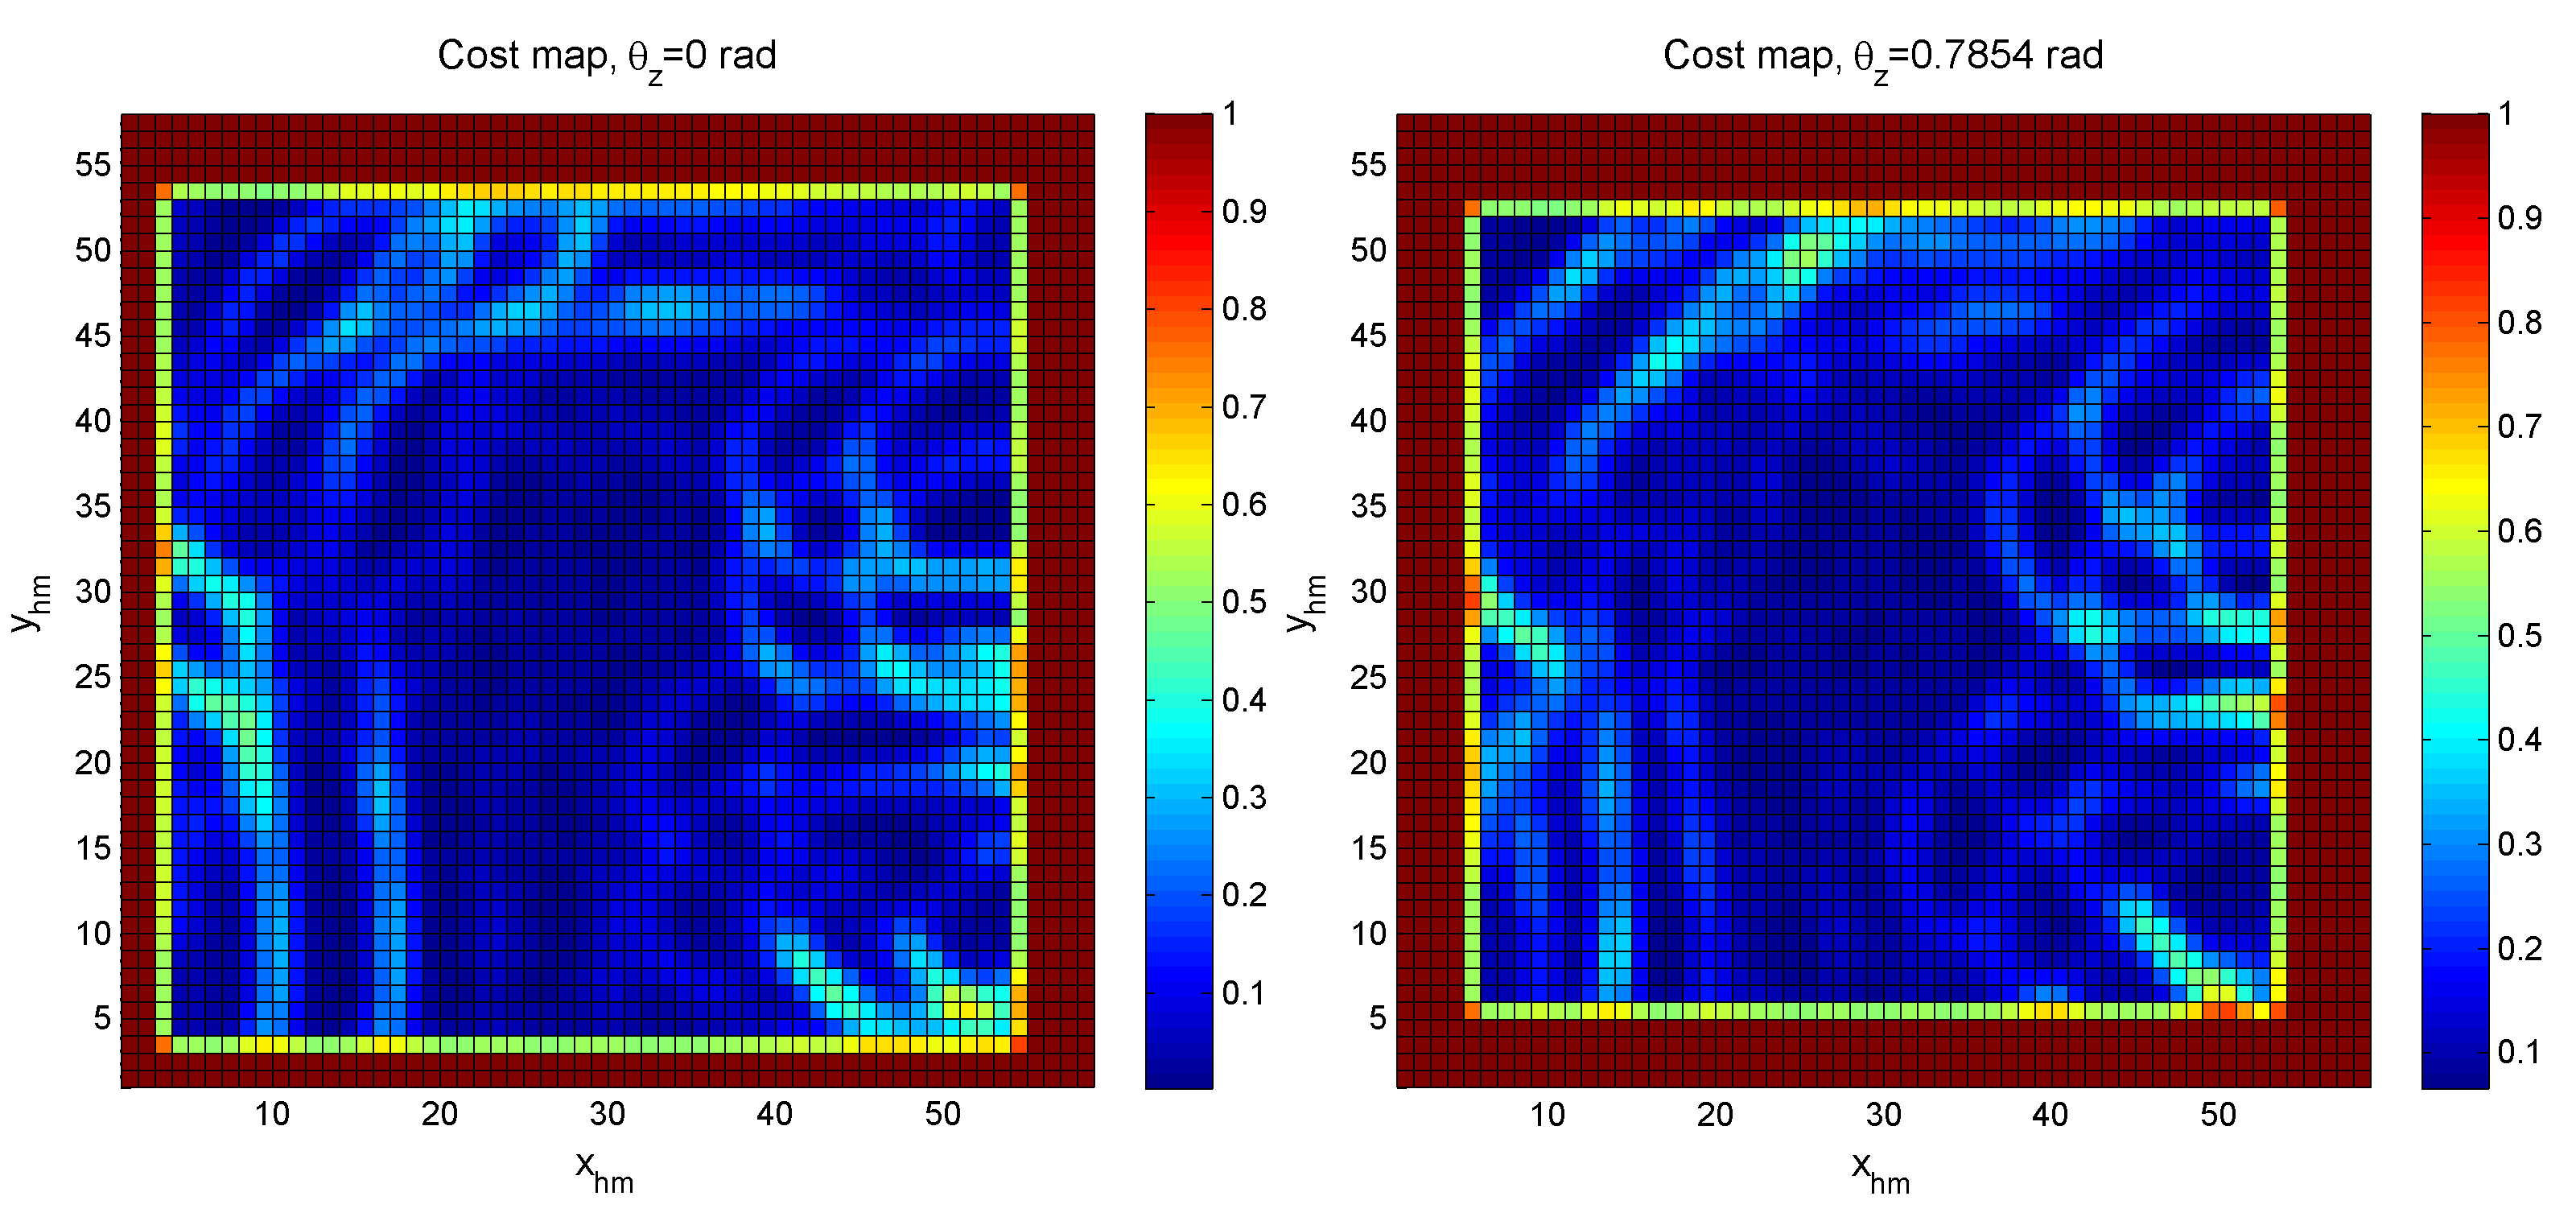
\includegraphics[width=1.00\textwidth]{cost_map.png}}
					\caption{Projections of a sample cost-tensor generated from the height-map shown in Figure~\ref{fig::heightmap_terrain_patch}.}
					\label{fig::cost_map}
				\end{figure}

			$\mmathcal{C}$ is used to generate an optimal, $N$-step path, which is comprised of $N$ discrete robot configurations. Moreover, the problem of planning a path over rough terrain is setup as a minimization of an $N$-step cost functional defined as follows:
				\begin{equation}			
					J(N) = \sum_{k=0}^N \mmathcal{C}\wrap{\bar{p}^{\mmathcal{M}}_{b,k},u_{k}}
				\end{equation}
			Here, $\mmathcal{C}\wrap{\bar{p}^{\mmathcal{M}}_{b,k},u_{k}}$ plays the role of a tabular objective function. An optimal path can be found from $\mmathcal{C}$ using an $A^{*}$-based path planning algorithm, for example \cite{Hart1968}. This method has yet to be fully explored in the scope of this project, but is widely accepted as a standard technique for optimal path planning in discrete spaces. Here, a sub-optimal approach is taken, which will be presented next.  Paths generated using the cost-tensor $\mmathcal{C}$ can be mapped back into $O_{0}$ using the corresponding inverse mappings of \ref{eq::toheightmapframe} and $\gamma\wrap{u}$, and interpolated to generate smooth trajectories.
			






		\subsection{A Sliding-Window Approach for Sub-Optimal Rough Terrain Planning}

			A sub-optimal planning algorithm is formulated as a preliminary method for terrain planning using the cost-tensor $\mmathcal{C}$. In this algorithm, navigation way-points are generated through a series of successive optimizations upon finite windows of  $\mmathcal{C}$. Each optimization step is used to plan a body position $\bar{p}^{\mmathcal{M}}_{b,k}$ way-point and an orientation $u_{k}$, starting from an arbitrary initial position, $\bar{p}^{\mmathcal{M}}_{b,0}$ and orientation $u_{0}$. Each optimization step takes the form:
				\begin{equation}
					\begin{split}
							&	\min_{\psi_{k},\lambda_{k}}\mmathcal{C}\wrap{\psi_{k},\lambda_{k}} 	\\
					\text{s.t. }	\psi_{k}&\in\mmathbb{Z}^{w}_{k}							\\
									\lambda_{k}&\in\mmathbb{Z}^{u}_{k}
					\end{split}
					\label{eq::local_min}
				\end{equation}
			where $\psi_{k}=\{i_{\psi,k},j_{\psi,k}\}$; and $\mmathbb{Z}^{w}_{k}\subset\mmathbb{Z}^{\mmathcal{M}}$ and $\mmathbb{Z}^{u}_{k}\subset \{ 1,...,l \}$ are moving, asymmetric windows about each $(k-1)^{th}$ way-point position and orientation, respectively, defined as follows:
				\begin{equation}
					\begin{split}
						\mmathbb{Z}^{w}_{k} & \text{ s.t.}  \\
						i_{\psi,k} 	& \in \{ \wrap{i_{b,k-1}-d_{w}},\wrap{i_{b,k-1}-d_{w}+1},...,\wrap{i_{b,k-1}+d_{w}} \} 	\\
						j_{\psi,k} 	& \in \{ \wrap{j_{b,k-1}+1},...,\wrap{j_{b,k-1}+d_{w}} \} 	\\
						\mmathbb{Z}^{u}_{k}	&=   \{ \wrap{u_{k-1}-d_{u}}, \wrap{u_{k-1}-d_{u}+1}, ... , \wrap{u_{k-1}+d_{u}} \}
					\end{split}
					\label{eq::windows}
				\end{equation}			
			with $\psi_{k} = \wrap{i_{\psi,k},i_{\psi,k}}$; $p_{b,k-1}^{\mmathcal{M}} = \wrap{i_{b,k-1},j_{b,k-1}} \in \mmathbb{Z}^{\mmathcal{M}}$, as previously defined; and $d_{w}>0$ and $d_{u}>0$ being integer window-size parameters. The asymmetry of these windows in the $j_{\psi,k}$ coordinate direction ensures that the \Kth way point is planned forward from the $(k-1)^{th}$ way-point in the $y$-axis direction (\IE such that there is no back-tracking). The local optimizers $\psi_{k}^{*}$ and $\lambda_{k}^{*}$, represent the coordinates at which the objective function in \ref{eq::local_min} is minimized. They are used to generate a \Kth trajectory way-point by:
				\begin{equation}
					\begin{split}
						i_{b,k} &= i_{b,k-1} 	+ \text{sign}(i_{\psi,k}^{*} -d_{w}/2 - 1) 	\\
						j_{b,k} &= j_{b,k-1} 	+ \text{sign}(j_{\psi,k}^{*}-1) 			\\
						u_{k} 	&= u_{k-1} 		+ \text{sign}(\lambda_{k}^{*}-d_{u}/2-1) 	\\
					\end{split}
				\end{equation}
			where $\text{sign}(n)$ is an operator such that:
				\begin{equation}
					\text{sign}(n) =
					\begin{cases}
							+1 &	\text{if } n > 0 \\
						    -1 &	\text{otherwise}
					\end{cases}
				\end{equation}

			Figures~\ref{fig::terrain_path_1} through \ref{fig::terrain_path_4} show simulated path-planning results over the terrain originally depicted in Figure~\ref{fig::pointcloud_terrain_patch}. Simulations were configured such that a path is planned from a starting point near the $y=0$ in the real-world coordinate from, to the opposite side of the terrain patch moving in the $y$-axis direction. In each simulation group, the $x$-coordinate of the initial position $p_{b,0}^{0}$ and initial orientation, $u_{0}$, are varied for each trial. A single window size for $d_{w}$ and $d_{u}$ is configured for each simulation group. The resulting planned paths are displayed with respect real-world coordinates, mapped from the $O_{\mmathcal{M}}$ frame. Each planned path is smoothed using a moving-average filter. Table~\ref{tab::cost_tabulation} summarizes the total cost of each path taken for each trial, with respect to a selected window size. 

				\begin{table}
					\centering
					\begin{tabularx}{\textwidth}{|C{0.25}||C{0.15}|C{0.15}|C{0.15}|C{0.15}|C{0.15}|}\hline
									& 	\textbf{T1}		&	\textbf{T2} &	\textbf{T3} &	\textbf{T4} \\ \hline \hline
						$d_{w}=d_{u}=1$ 	&	24.9012		& 	25.1534	& 	28.9889	& 	29.9231	\\ \hline
						$d_{w}=d_{u}=5$ 	&	20.2524		& 	21.8537	& 	23.8874	& 	20.7319	\\ \hline
						$d_{w}=d_{u}=15$ 	&	16.8602		& 	21.8307	& 	19.4236	& 	23.5314	\\ \hline
						$d_{w}=d_{u}=30$ 	&	19.3791		& 	19.0536	& 	23.6496	& 	23.6142	\\ \hline
					\end{tabularx}
					\caption{Sum of costs for four path-planning trials with varying initial positions varying optimization windows.}
					\label{tab::cost_tabulation}
				\end{table}		

				\begin{figure}
					\centering
					\fbox{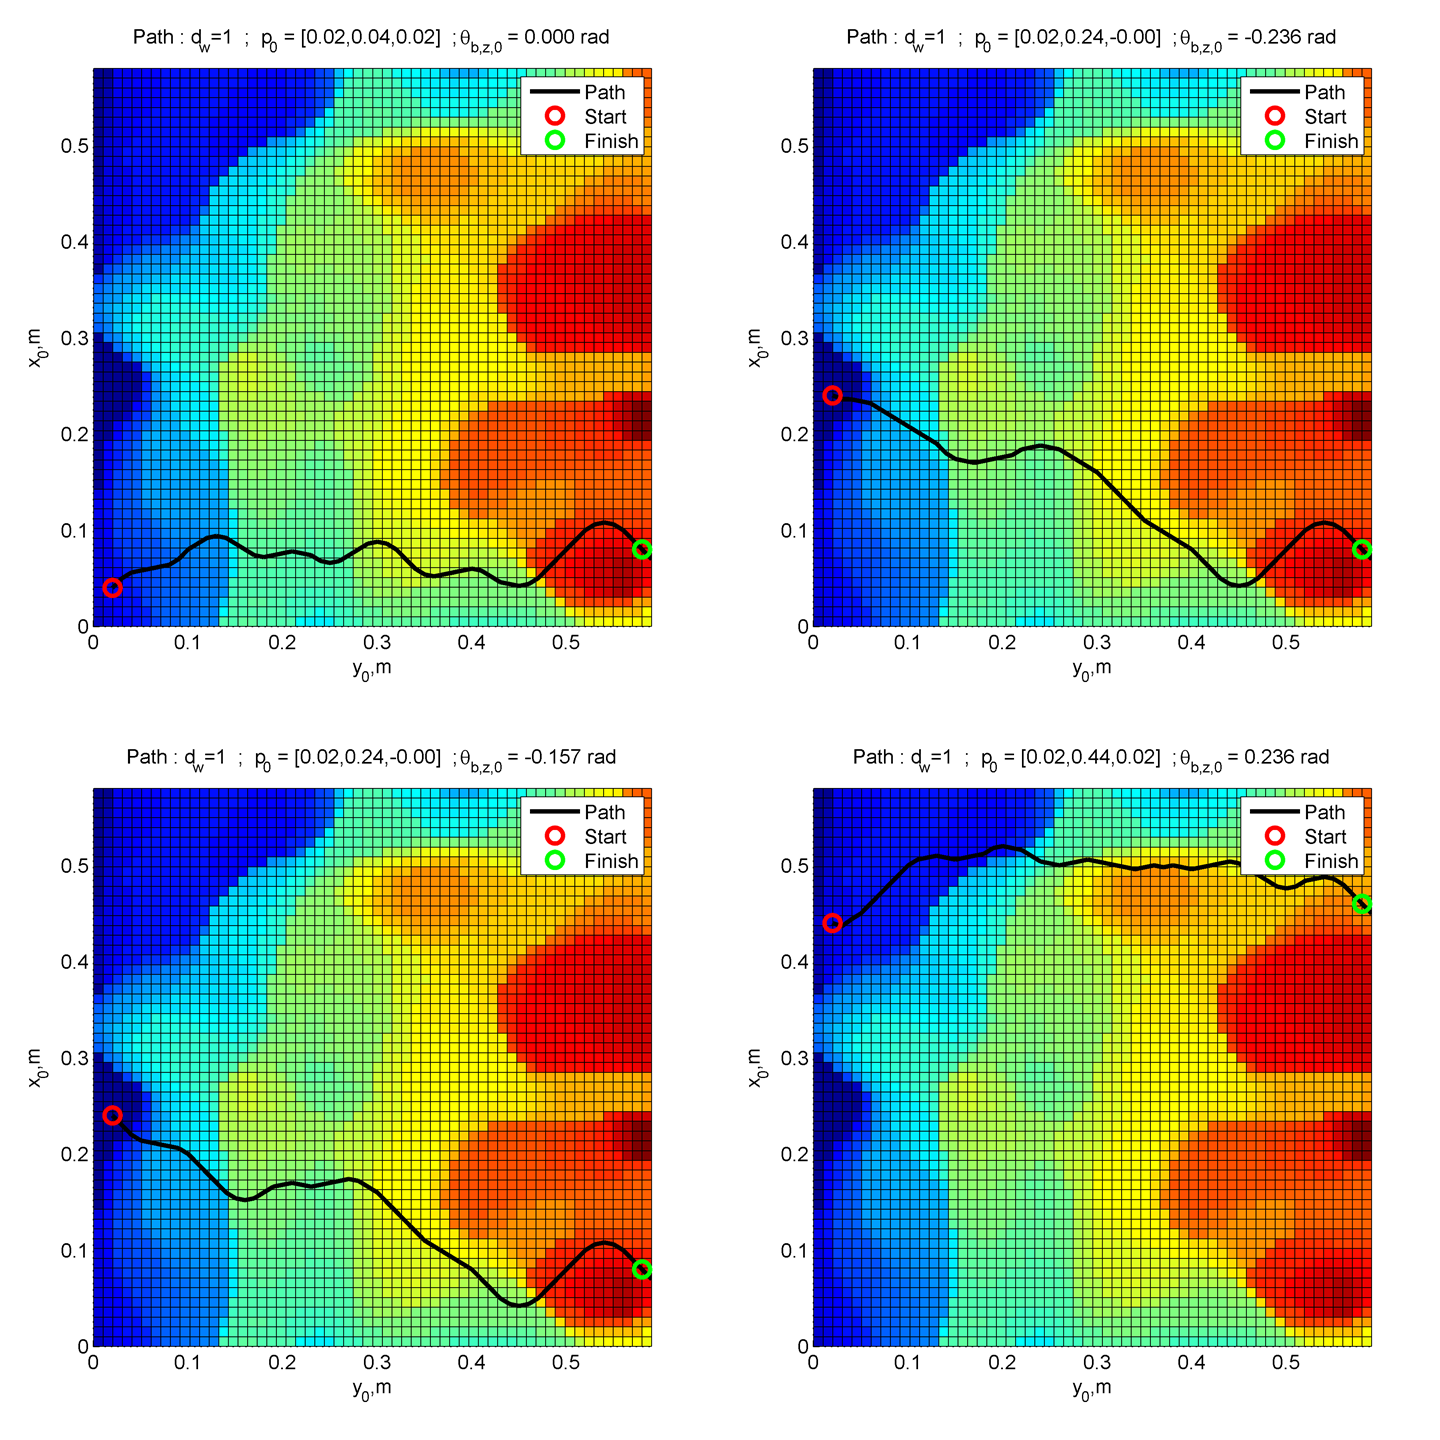
\includegraphics[width=1.00\textwidth]{terrain_path_1.png}}
					\caption{Path planned over rough terrain with $d_{w}=d_{u}=1$.}
					\label{fig::terrain_path_1}
				\end{figure}
				\begin{figure}
					\centering
					\fbox{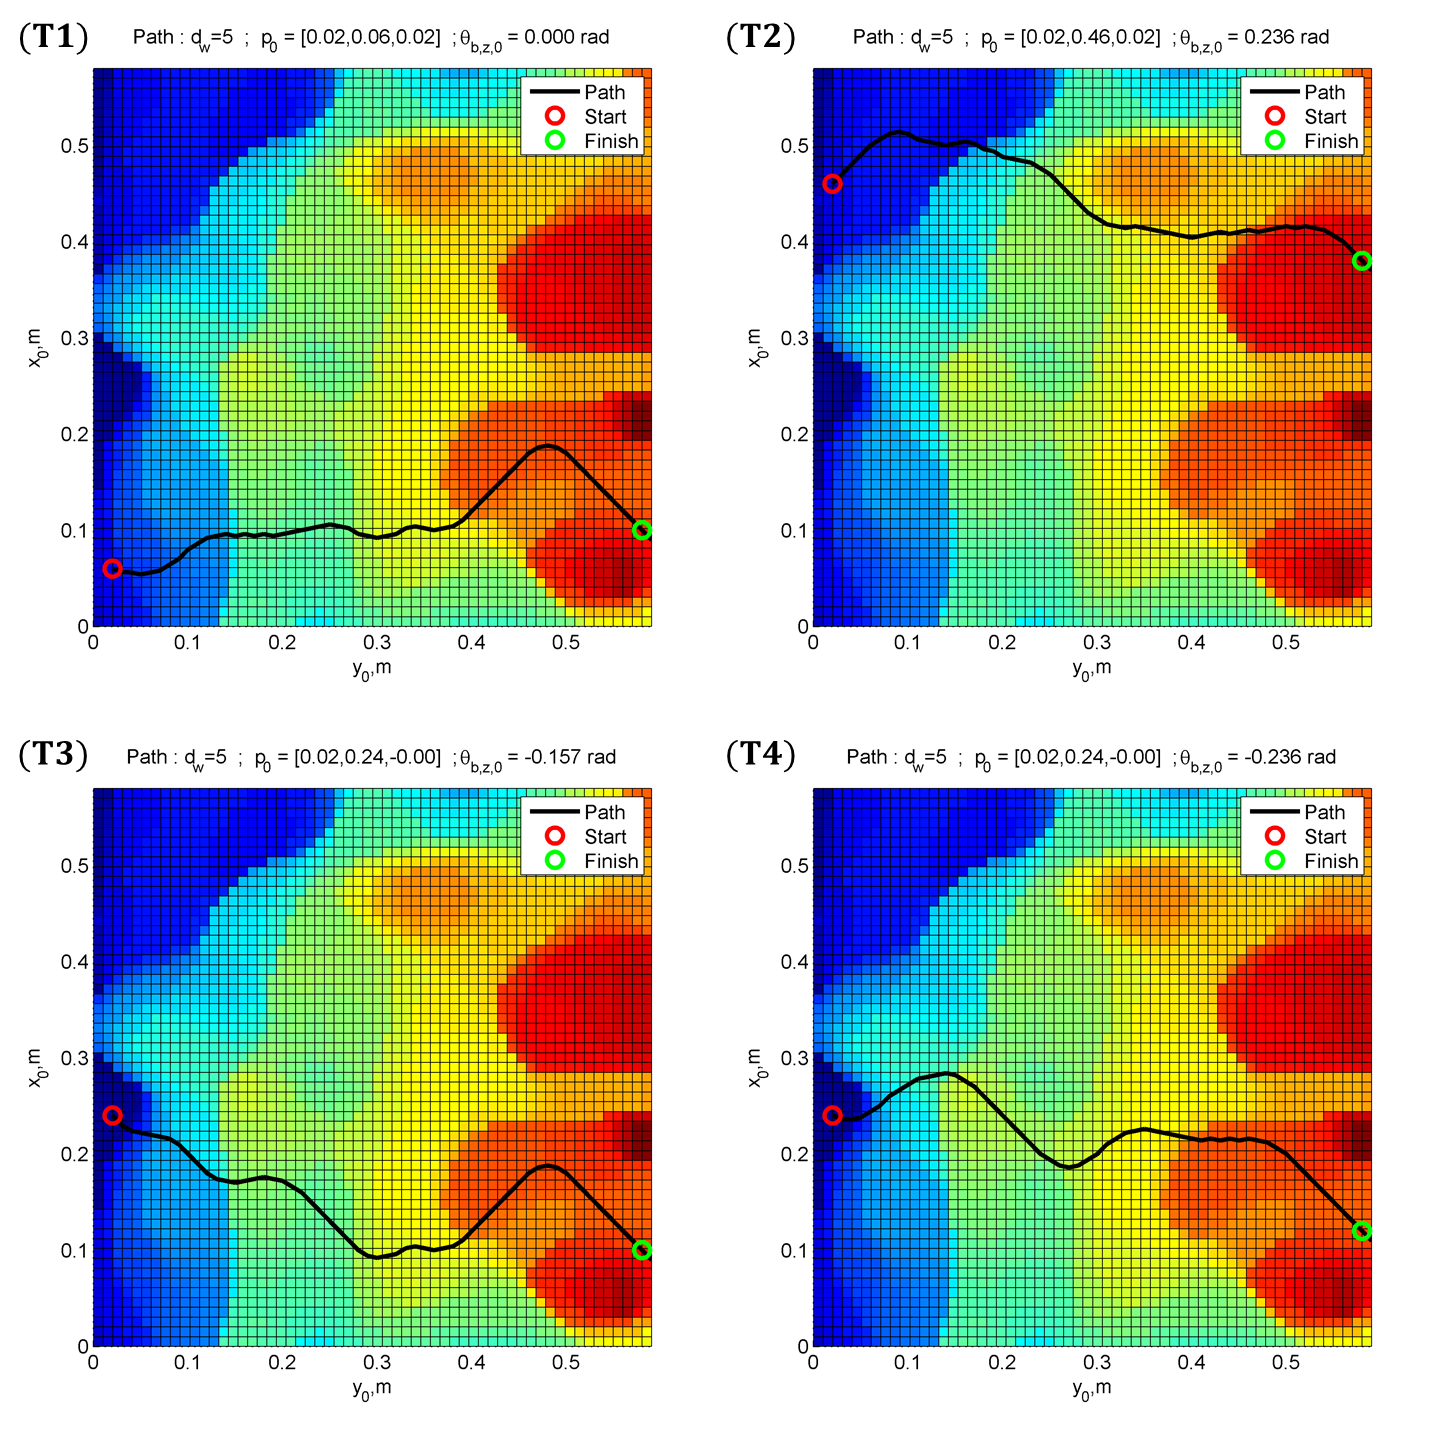
\includegraphics[width=1.00\textwidth]{terrain_path_2.png}}
					\caption{Path planned over rough terrain with $d_{w}=d_{u}=5$.}
					\label{fig::terrain_path_2}
				\end{figure}
				\begin{figure}
					\centering
					\fbox{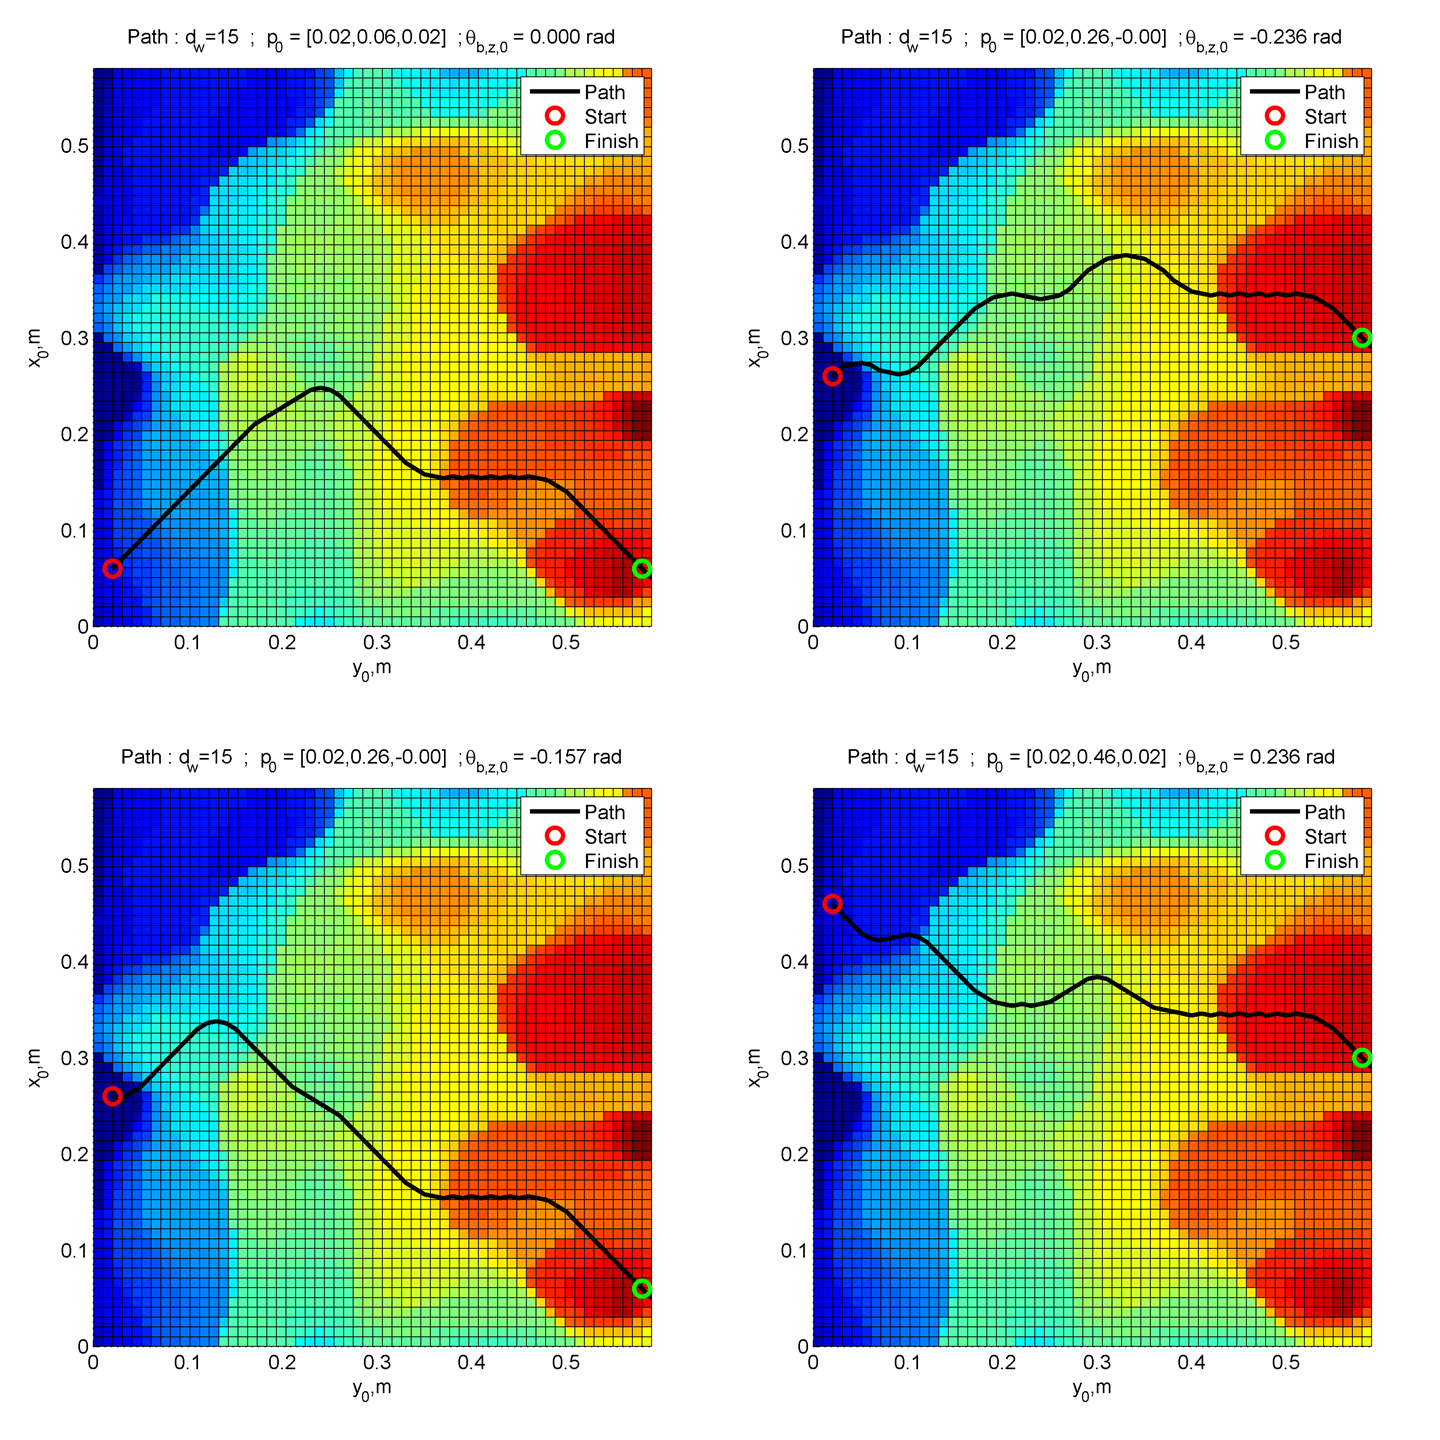
\includegraphics[width=1.00\textwidth]{terrain_path_3.png}}
					\caption{Path planned over rough terrain with $d_{w}=d_{u}=15$.}
					\label{fig::terrain_path_3}
				\end{figure}
				\begin{figure}
					\centering
					\fbox{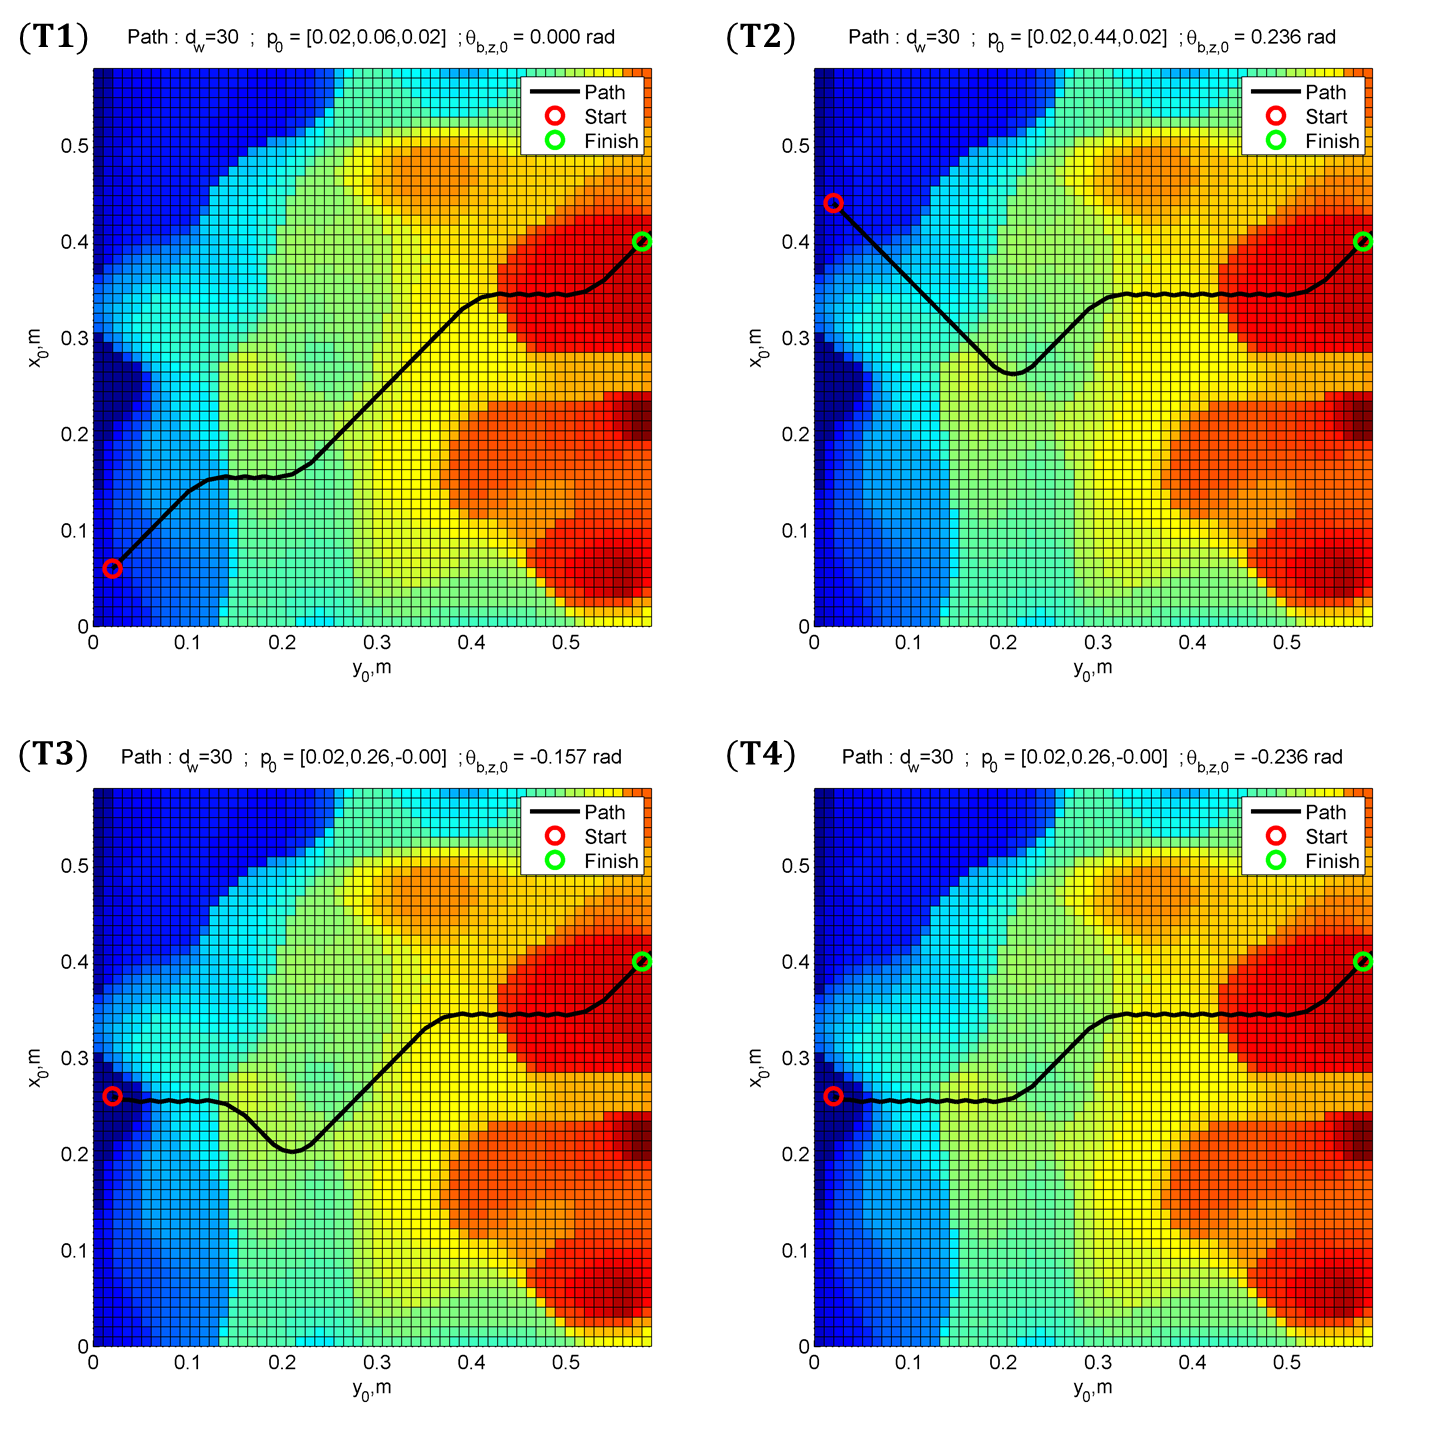
\includegraphics[width=1.00\textwidth]{terrain_path_4.png}}
					\caption{Path planned over rough terrain with $d_{w}=d_{u}=30$.}
					\label{fig::terrain_path_4}
				\end{figure}



		\subsection{Surface Reconstruction}

			3D surface reconstruction is carried out according to a process for normal-estimation detailed in \cite{Rusu2009}. According to this procedure, 3D surfaces are reconstructed from point cloud, $\bar{S}$, by fitting a collection of flat polygonal elements to successive point clusters which fall within a range $d_{s}$ of each point in $\bar{x_{i}}\in\bar{S}$. Each of these estimated elements is represented by a surface-normal which emanates from each $\bar{x_{i}}$ within the source cloud.

			The raw 3D point cloud, $\bar{S}$, which is typically dense, is down-sampled and smoothed before a normal estimation algorithm is applied. Point cloud down-sampling is performed using a voxel-grid technique, which discretizes the point cloud space into a voxel-space. The voxel-space consists of stacked cuboids of a particular side-length. Each cubic unit of the voxel space is parameterized by a single voxel side-length dimension $d_{vox}$. The voxel-grid filter generates a single-point from all points which fall within a voxel region. A KD-tree search technique is used to find points which are contained by a particular voxel region. This technique offers higher efficiency over a brute-force search for neighboring points. This voxel-grid down-sampling technique produces a reduced representation of the original cloud, $\hat{S}$. Empirical results have shown that $\hat{S}$ can contain up to ten to twenty times less points than the original cloud, $\bar{S}$. This reduced-point cloud representation greatly reduces the computational effort needed to process the point cloud $\hat{S}$.
			
			\begin{algorithm}
				\begin{algorithmic}
					\State{\textbf{init} $\hat{S},\bar{S},\bar{S}^{*},d_{vox},\vec{u}^{r},e,e_{max}$}
					\State{$\hat{S} = \text{voxelGridFilter}(\bar{S},d_{vox})$}
					\State{$\hat{S} \leftarrow \text{movingLeastSquaresFilter}(\hat{S})$}
					\State{$\hat{N} = \text{estimateNormals}(\hat{S})$}
					\ForAll{$\vec{n}_{i} \in N$}
						\State{$e = 1-(\vec{u}^{r})^{T} \vec{n}_{i}$}
						\If{$e<e_{max}$}
							\State{ $\bar{S}^{*} \leftarrow \bar{S}^{*} \cup \bar{x}_{i}$ }
						\EndIf
					\EndFor
				\end{algorithmic}	
				\caption{Finding good places to step from a 3D point cloud.}
				\label{alg::goodspacestostep}
			\end{algorithm}

			Next, the resulting cloud, $\hat{S}$, is regularized using a moving least-squares filter. This filter creates a smoothed point cloud by performing a sequence polynomial fits over a moving subset of points. Once regularized, normals are estimated from the point cloud via a plane fitting method, as described in \cite{Mitra2003}. Planes are estimated using Principle Component Analysis (PCA) on clusters of points \cite{Castillo2013}. The standard PCA algorithm provides a least-squares plane fit by way of dimensional reduction, yielding best-fit description for a set 3D points as a 2D manifold \cite{Pearson1901}. The full surface-normal estimation algorithm is provided in Algorithm~\ref{alg::normal_estimation}. A point cloud with estimated surface normals is shown in Figures~\ref{fig::surface_estimation} and \ref{fig::surface_estimation2}.

			Algorithm~\ref{alg::goodspacestostep} is used convert a 3D point cloud into an augmented point-cloud with normal vectors. This augmented cloud is then used to find ``flat" regions within the reconstructed surface. This is performed for the purpose of footstep planning. Flat regions are located using the computed surface normals. The alignment of each \Ith normal, $\vec{n}_{i}$, is compared to a reference unit vector, $\vec{u}^{r}$, by taking a dot product. This dot-product operation produces an alignment error $e\in[0,2]$. Points with associated normals whose alignment error is less than a scalar error bound, $e_{max}$, are selected as surfaces fit for walking (\IE flat). Obviously, not all surfaces which satisfy this alignment criteria represent surfaces which are fit for traversal. Beyond normal estimation, several additional post processing operations are necessary. Namely, the resulting point cloud must be segmented into regions which are traversable by the robot.

			\begin{figure}[!h]
				\centering
				\fbox{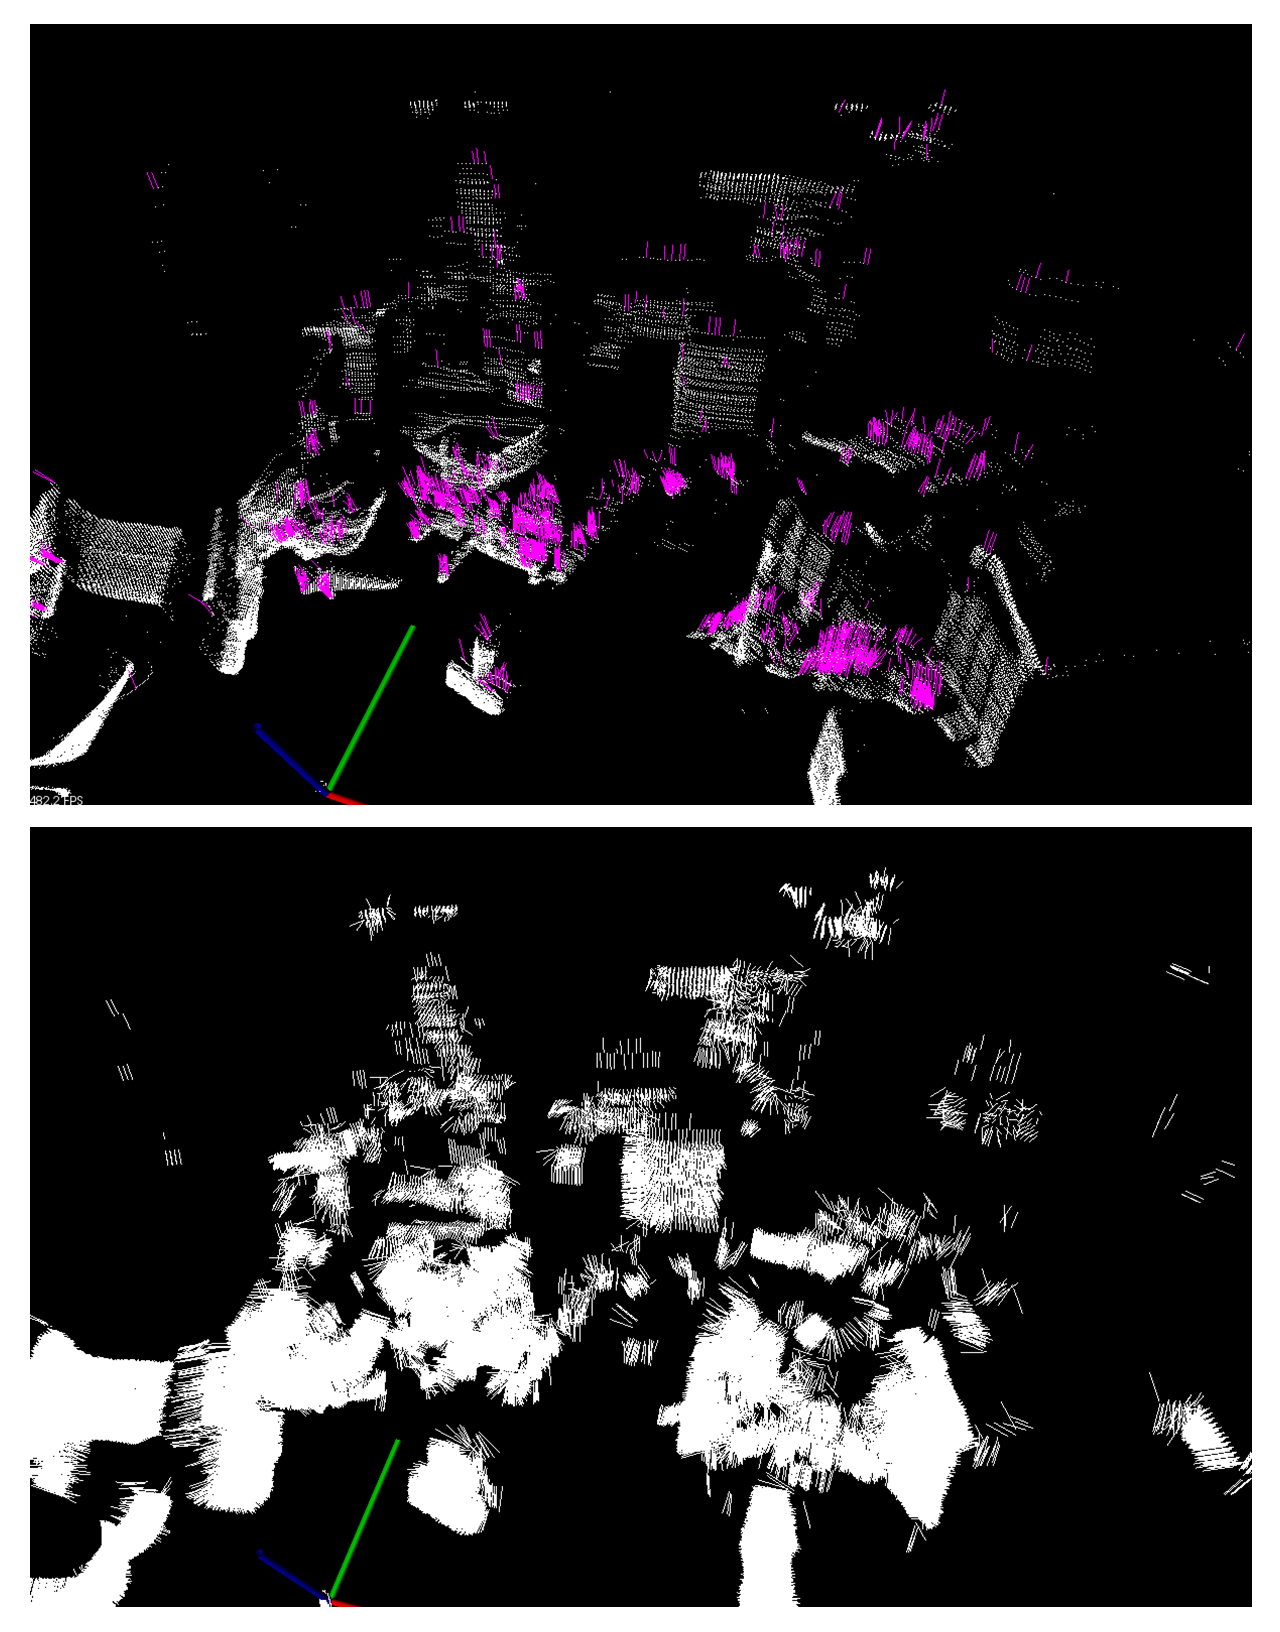
\includegraphics[width=\textwidth]{surf_reconstruction.png}}
				\caption{Point cloud generated from sequential scans of a room showing flat-surface candidates \emph{(top)} and 3D point cloud with estimated normals \emph{(bottom)}.}
				\label{fig::surface_estimation}
			\end{figure}
			\begin{figure}[!h]
				\centering
				\fbox{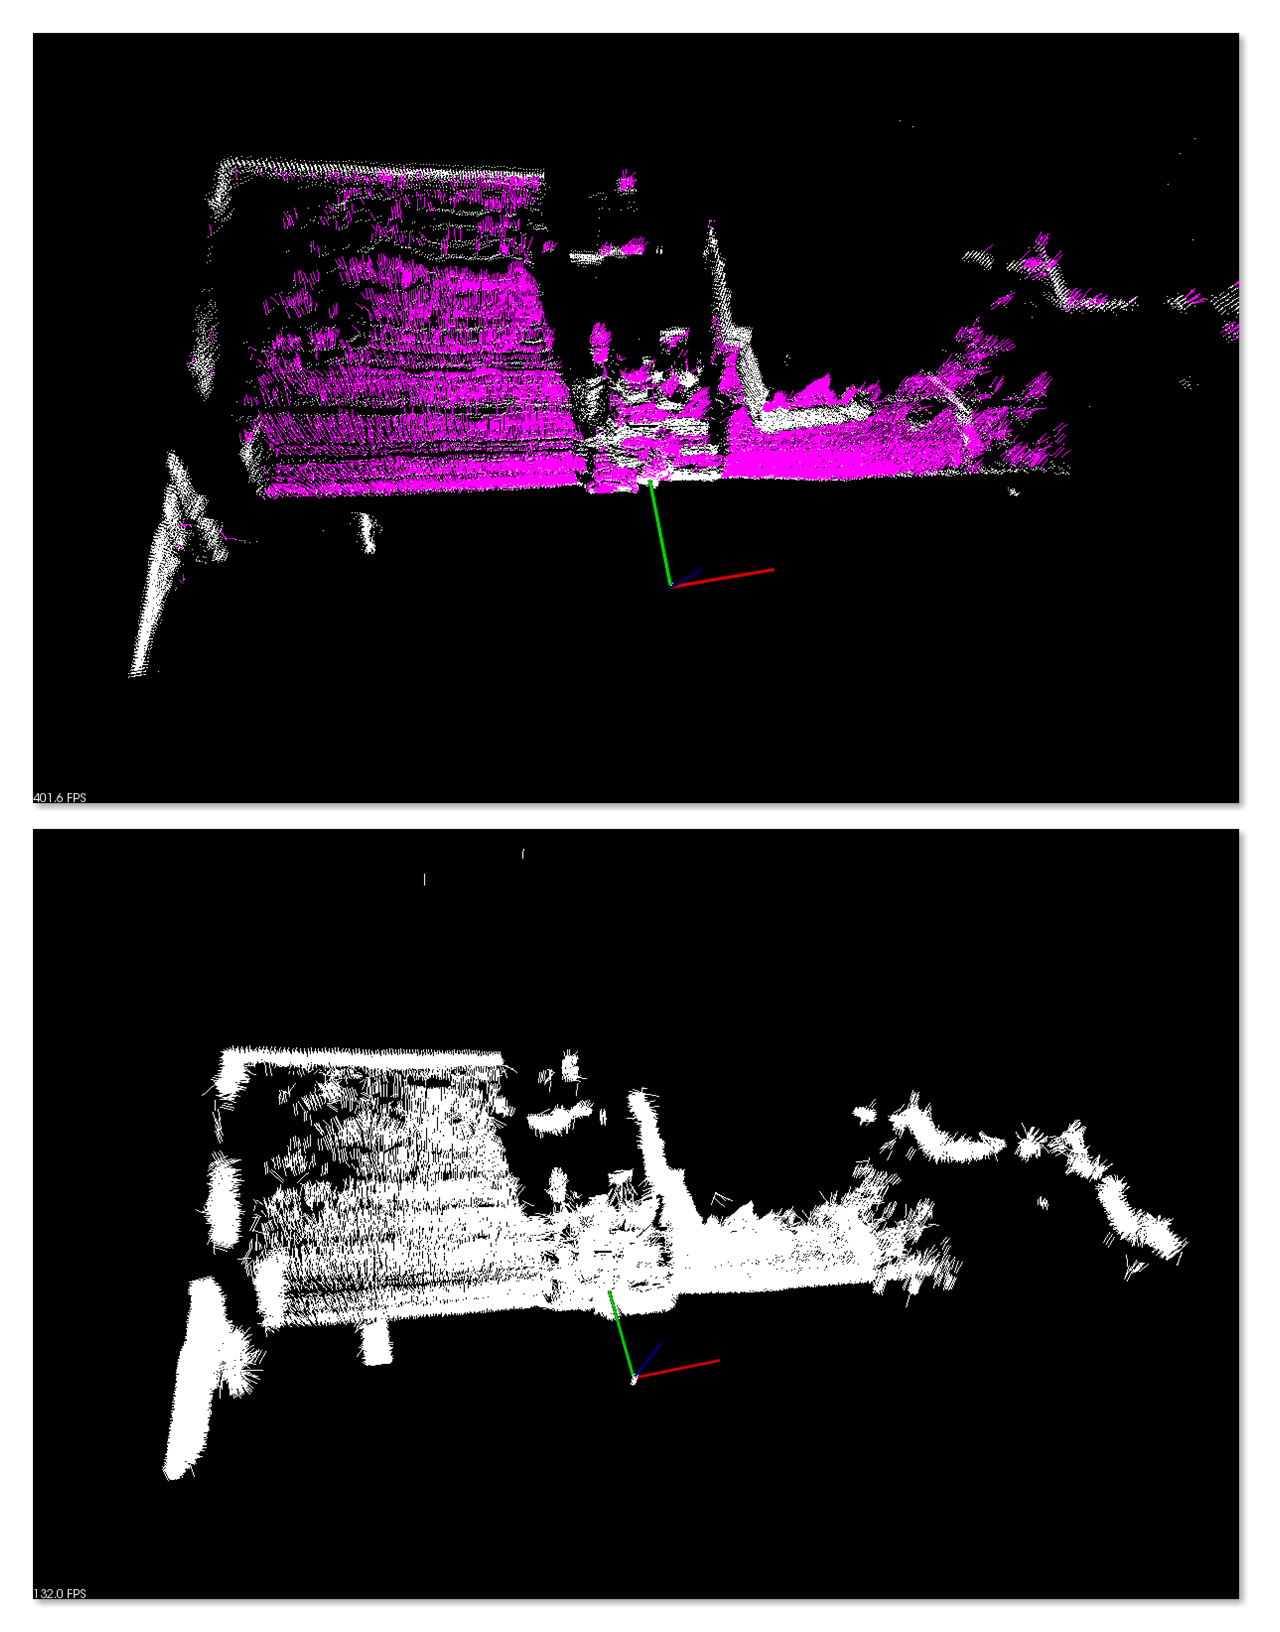
\includegraphics[width=\textwidth]{surf_reconstruction2.png}}
				\caption{Point cloud generated from sequential scans of a floor with obstacles showing flat-surface candidates \emph{(top)} and 3D point cloud with estimated normals \emph{(bottom)}.}
				\label{fig::surface_estimation2}
			\end{figure}
			%C++ implementations for the aforementioned surface reconstruction algorithms using the OpenPCL framework have been included in Appendix~\ref{appendix::d}.